\documentclass[11pt]{article}
\usepackage[margin=0.75in,top=0.7in,bottom=0.7in]{geometry}
\usepackage{graphicx,amsmath,amssymb,booktabs,array,xcolor}
\usepackage{fancyhdr,titlesec,enumitem,caption,float}
\usepackage[T1]{fontenc}
\usepackage[colorlinks=true,linkcolor=blue,urlcolor=blue,citecolor=blue]{hyperref}

\captionsetup{font=small,labelfont=bf}
\setlist{itemsep=1pt,topsep=2pt,parsep=0pt}
\titlespacing*{\section}{0pt}{9pt}{4pt}
\titlespacing*{\subsection}{0pt}{7pt}{3pt}
\pagestyle{fancy}\fancyhf{}
\lhead{}\rhead{\small SERF-MAD Feasibility -- SR}
\cfoot{\small\thepage}
\renewcommand{\headrulewidth}{0.4pt}

\newcommand{\band}{\begin{center}\rule{\linewidth}{0.8pt}\end{center}}
\newcommand{\nT}{\,nT}\newcommand{\pT}{\,pT}\newcommand{\fT}{\,fT}

\begin{document}
\thispagestyle{fancy}
\band
\begin{center}
{\large\bfseries Feasibility of a Ruggedised SERF MEMS Vapour-Cell Magnetometer\\[2pt]
for Magnetic Anomaly Detection from an Autonomous Underwater Vehicle}\\[8pt]
{\normalsize Physics Modelling, GPU-Accelerated Simulation, and Component Requirements}\\[10pt]
{\small Scientific Report}\\[8pt]
{\small 15 August 2026}
\end{center}
\band
\vspace{-0.35cm}

\section*{Executive Summary}
\noindent Magnetic anomaly detection (MAD) is the one underwater sensing modality
unaffected by acoustic quieting, thermoclines, or multipath. Its historic
limitation has been sensitivity: detecting a small, deliberately demagnetised
object means resolving field perturbations far below the Earth's field.
Spin-exchange relaxation-free (SERF) atomic magnetometers now match or exceed
SQUID sensitivity without cryogenics \cite{allred2002,kominis2003,dang2010},
and microfabricated MEMS vapour cells make them small and mechanically robust
enough to consider for an autonomous underwater vehicle (AUV)
\cite{griffith2010,shah2007}.

This report assesses that concept from first-principles physics. A validated
simulation framework models the sensor quantum-mechanically, the target
electromagnetically, the vehicle kinematically, and detection statistically.
Twenty-seven independent verification, validation and stress tests all pass.

\textbf{The concept is physically sound, and the limiting factors are not where
intuition places them.} Sensor sensitivity is not the constraint --- it exceeds
requirement by five orders of magnitude. Two other factors govern feasibility:

\begin{enumerate}[leftmargin=1.5em]
\item \textbf{Ambient-field control sets the entire design.} SERF operation
requires the residual static field at the vapour cell to stay within a few
nanotesla \cite{borna2022}, against an ambient of $50{,}000\nT$
\cite{ncei}. Accounting for the Cross-Axis Projection Error (CAPE)
\cite{borna2022}, the true requirement derived here is $\leq 0.94\nT$: $94$~dB
of combined shielding and active nulling, and $5.3\times$ tighter than the
figure usually quoted.
\item \textbf{The system is clutter-limited, not sensor-limited.} Residual
platform interference measured on a real UUV exceeds MEMS-cell sensor noise by a
factor of $10^{5}$ \cite{oehler2024,griffith2010}. Improving the magnetometer
yields nothing; improving vehicle magnetic cleanliness, gradiometer rejection,
and compensation yields range almost proportionally.
\end{enumerate}

Predicted detection ranges at $P_{fa}=10^{-4}$, marginalised over unknown target
orientation, are $22$~m for a low-signature micro-UUV, $68$~m for a naval mine,
and $267$~m for a degaussed submarine. Section~8 states the component-level
requirements this implies; Section~9 sets out the barriers candidly.

\section{Introduction and Background}
\subsection{Why magnetic anomaly detection}
Any object containing ferromagnetic material distorts the local geomagnetic
field. A submarine, a mine, or a piece of unexploded ordnance carries both a
\emph{permanent} magnetisation acquired during construction and an
\emph{induced} magnetisation proportional to the ambient field
\cite{tolles1950,gnadt2022}. Beyond roughly one body length the combined effect
is well described by a magnetic dipole of moment $\mathbf{m}$ \cite{jackson1998},
producing
\begin{equation}
\mathbf{B}(\mathbf{r})=\frac{\mu_0}{4\pi}\,
\frac{3\hat{\mathbf{n}}(\mathbf{m}\cdot\hat{\mathbf{n}})-\mathbf{m}}{r^{3}} .
\label{eq:dipole}
\end{equation}
The $r^{-3}$ dependence is the defining practical fact of MAD: halving the
standoff increases signal eightfold, so detection range grows only as the cube
root of sensitivity. This is why MAD has always been a close-in sensor, and why
platforms that can approach the target --- aircraft historically
\cite{tolles1950,gnadt2022}, AUVs now \cite{oehler2024,seidel2023} --- matter
more than incremental sensor improvements.

The compensating advantage is that magnetostatic fields are indifferent to the
acoustic environment. Hull quieting, anechoic coatings, thermoclines, biologics
and shipping noise all degrade sonar but not magnetics. Against modern quiet
submarines, and against small non-emitting objects such as seabed munitions
\cite{seidel2023,oehler2024}, a magnetic channel is genuinely complementary
rather than redundant.

\subsection{The sensitivity problem, and how atomic magnetometers solve it}
Consider a low-signature target of moment $5$~A$\cdot$m$^2$ at $20$~m.
Equation~\eqref{eq:dipole} gives roughly $25\pT$ --- about two parts in $10^{6}$
of the Earth's field \cite{ncei}. Fluxgate magnetometers, the traditional
workhorse of marine survey, are typically deployed where anomalies of order
$10\nT$ and above must be resolved \cite{oehler2024}; a picotesla-class target
sits well beyond routine fluxgate capability before platform noise is even
considered. Historically only superconducting quantum interference devices
(SQUIDs) offered materially better resolution \cite{budker2007,clem1997}, at the
cost of liquid helium and a cryostat: workable on a large aircraft, unattractive
on a small autonomous vehicle.

Optically pumped atomic magnetometers instead measure field by observing how fast
atomic spins precess \cite{budker2007}. A vapour of alkali atoms (rubidium,
potassium or caesium) is optically pumped by a circularly polarised laser so the
electron spins align along the beam; a magnetic field perpendicular to that axis
torques the spins, and the resulting rotation is read out through the
polarisation of a probe beam via Faraday rotation
\cite{griffith2010,seltzer2008}. The precession rate is set by the gyromagnetic
ratio $\gamma_e/2\pi\approx28$~Hz/nT \cite{wei2023,savukov2005}, a constant of
nature, so the instrument is intrinsically calibrated --- operationally valuable,
because a sensor that cannot drift out of calibration needs no field
recalibration between missions \cite{nist_micro}.

The classical obstacle was \emph{spin-exchange relaxation}. Alkali atoms collide
constantly, and each collision can exchange spin, randomising phase and
broadening the resonance \cite{happer1977,savukov2005}. Raising vapour density to
increase signal also increases collisions, so sensitivity saturated. The SERF
insight, demonstrated by Allred \emph{et al.} \cite{allred2002}, is that this
reverses in a specific regime: if the spin-exchange rate is made \emph{much
faster} than the Larmor precession rate, atoms exchange spin so rapidly that they
all sample the same average precession and the dephasing averages away
\cite{happer1977,savukov2005}. The requirement is high alkali density
\emph{and} very low field. Allred \emph{et al.} obtained a resonance linewidth of
$1.1$~Hz for potassium at $n=10^{14}$~cm$^{-3}$ and a sensitivity of
$10\fT/\sqrt{\rm Hz}$, limited by Johnson-current noise in the magnetic shields
rather than by the atoms, with an estimated shot-noise floor of
$2\times10^{-18}$~T$/\sqrt{\rm Hz}$ \cite{allred2002}. Kominis \emph{et al.}
subsequently demonstrated sub-femtotesla multichannel operation
\cite{kominis2003}, and Dang \emph{et al.} reached $0.16\fT/\sqrt{\rm Hz}$
\cite{dang2010}, better than any SQUID, with no cryogenics. The field is reviewed
in \cite{budker2007,li2018}.

\subsection{Why MEMS matters for a deployable sensor}
Laboratory SERF magnetometers use glass-blown centimetre-scale cells: fragile,
bulky, and unsuited to a vehicle experiencing launch shock, vibration and
pressure cycling. Microfabrication instead etches the vapour cavity into a
silicon wafer and seals it with anodically bonded glass windows
\cite{liew2004,schwindt2004}, producing a monolithic solid-state part of roughly
a cubic millimetre. Griffith \emph{et al.} \cite{griffith2010} demonstrated
$5\fT/\sqrt{\rm Hz}$ SERF operation in an $^{87}$Rb cell formed as a cavity
etched in a $1$~mm silicon wafer with anodically bonded Pyrex windows, with a
$1$~mm$^3$ measurement volume defined by the overlap of pump and probe beams near
$795$~nm; earlier microfabricated devices reached sub-picotesla performance
\cite{shah2007}. Anodic bonding forms a hermetic, essentially permanent
glass-to-silicon seal \cite{liew2004}; the structure has no moving parts and no
free volume, which is the core of the ruggedisation argument. This report adopts
the Griffith device as its design point.

\subsection{The hard part: this sensor dislikes the Earth}
The property that gives SERF its sensitivity --- operation at near-zero field
\cite{allred2002} --- is exactly what makes it difficult to deploy. Borna
\emph{et al.} \cite{borna2022} state that the SERF regime accommodates remnant
static magnetic fields only up to approximately $\pm5\nT$, while the Earth's field
spans $25{,}000$--$65{,}000\nT$ \cite{ncei}, so the field at the cell must be
actively cancelled. Unshielded and in-situ compensation schemes exist
\cite{seltzer2004,fang2012}, but all rest on reducing the residual to this window.

On a moving vehicle this is worse than it first appears. Even a perfectly constant
geomagnetic field becomes a large \emph{time-varying} field in the sensor's frame
as the vehicle rolls and pitches: a $3^{\circ}$ roll projects
$50{,}000\sin(3^{\circ})\approx2{,}600\nT$ onto a body axis. This is the same
mechanism that motivates aeromagnetic compensation \cite{tolles1950,gnadt2022}
and that limits wearable OPM systems during subject movement
\cite{boto2018,borna2022b}. The nulling system must therefore track a disturbance
that moves with the sea, not merely cancel a static offset. Quantifying that
requirement, and what it implies for hardware, is the central purpose of this
report.

\section{Scope and Objectives}
Figure~\ref{fig:setup} summarises what is modelled and why it is hard.

\textbf{Objective.} To determine from first-principles physics whether a
ruggedised SERF MEMS magnetometer is a credible AUV MAD payload, and to derive
the component-level requirements that follow.

\textbf{In scope.} SERF spin dynamics (open-quantum-system and semiclassical);
dipole target signatures and gradient tensors; AUV attitude dynamics; the
ambient-field nulling chain; platform interference compensation; matched-filter
detection and Monte Carlo performance; GPU-accelerated parameter sweeps; and
verification, validation and stress testing.

\textbf{Out of scope.} Optical subsystem design; vapour-cell fabrication
chemistry \cite{liew2004}; spin-squeezing schemes \cite{mitchell2020};
hydrodynamic design; classified signature data. Absolute sensitivity in
$\fT/\sqrt{\rm Hz}$ is not predicted (Section~9).

\begin{figure}[htbp]\centering
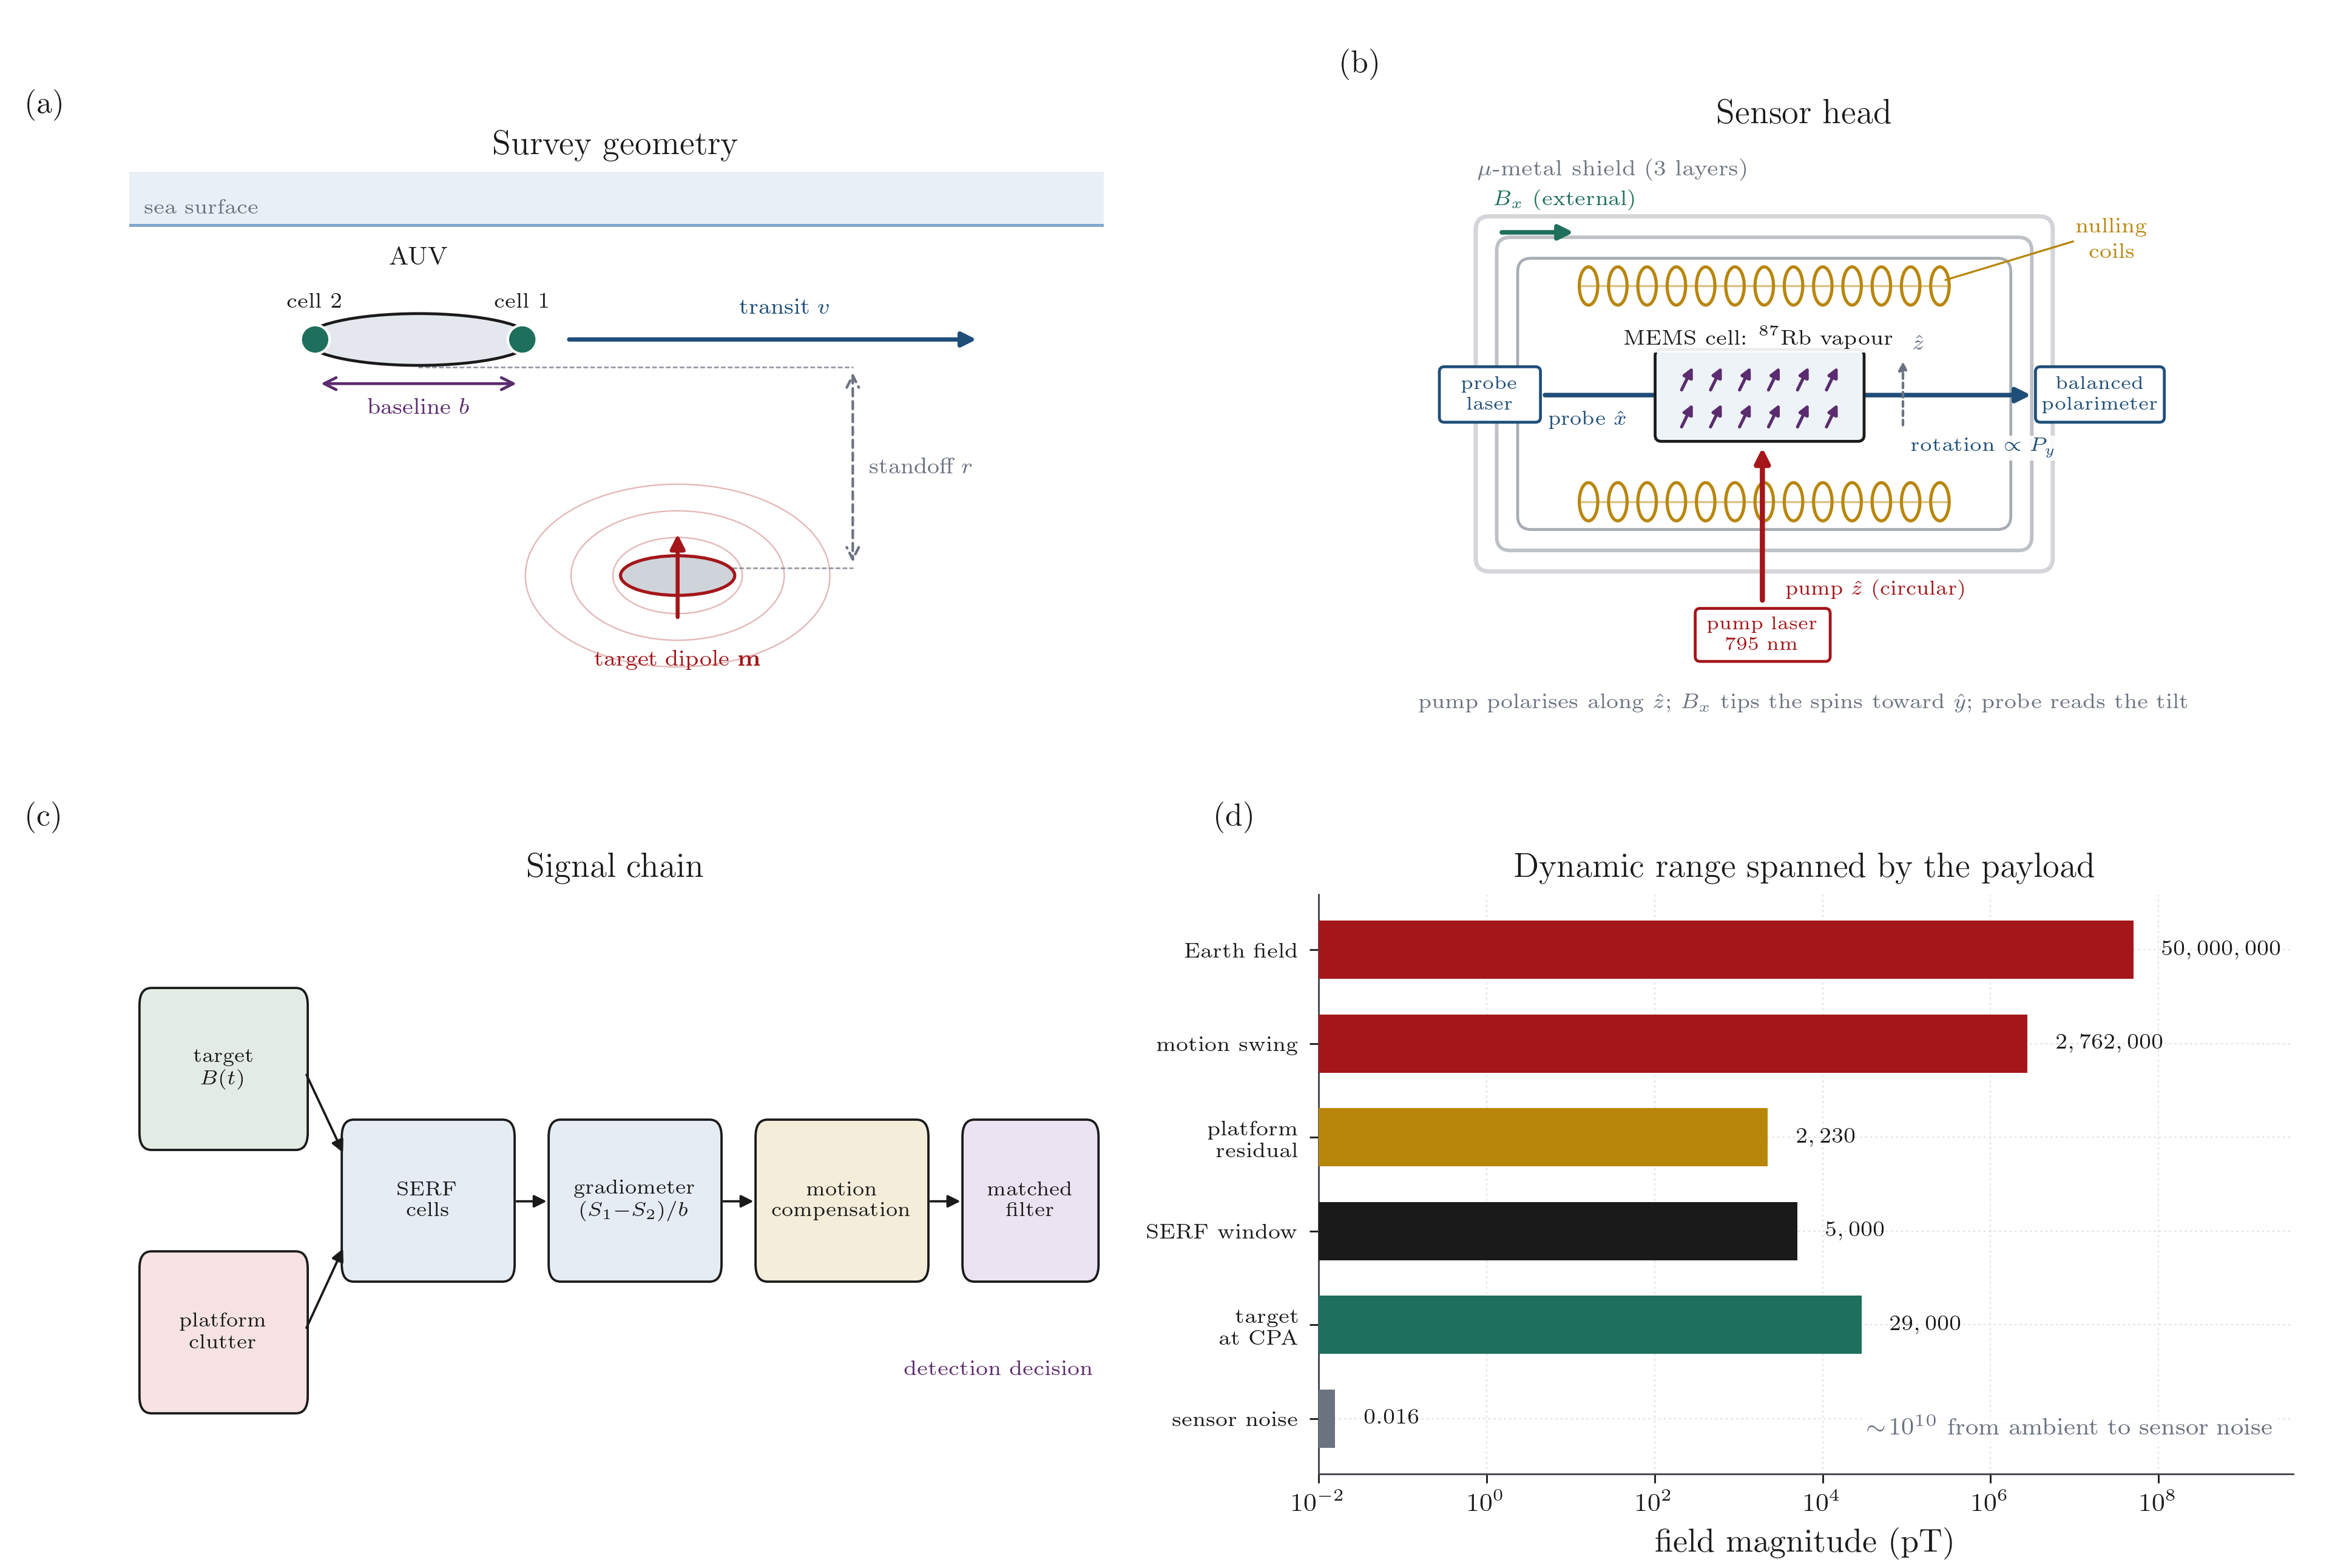
\includegraphics[width=0.86\linewidth]{outputs/fig_setup.png}
\caption{Simulation setup. (a) Survey geometry: the AUV transits above a dipole
target carrying two SERF cells on a rigid baseline. (b) Sensor head: the
microfabricated cell \cite{griffith2010} inside passive shielding and three-axis
nulling coils, optically pumped along $\hat z$ and probed along $\hat x$ so that
a transverse field is sensed as $P_y$. (c) Signal chain from field to detection
decision. (d) The dynamic range the payload must span --- roughly ten orders of
magnitude from the ambient geomagnetic field \cite{ncei} down to the MEMS sensor
noise floor \cite{griffith2010}, which is the central engineering difficulty
identified in this report.}
\label{fig:setup}
\end{figure}

\section{Physical Model}
\subsection{Sensor}
The spin ensemble is modelled at two fidelities. The reference model solves the
Lindblad master equation
$\dot\rho=-\tfrac{i}{\hbar}[H,\rho]+\sum_k\mathcal{D}[L_k]\rho$
\cite{lindblad1976,breuer2002} for a single effective spin-$\tfrac12$, with
collapse operators for optical pumping, spin destruction and dephasing,
integrated using QuTiP \cite{qutip2013}. The production model integrates the
phenomenological SERF Bloch equation for the ensemble-averaged polarisation
$\mathbf{P}=2\langle\mathbf{S}\rangle$ \cite{seltzer2008,borna2022},
\begin{equation}
\frac{d\mathbf{P}}{dt}=\frac{1}{q}\Big[\gamma_e(\mathbf{P}\times\mathbf{B})
+R_{op}(\hat{\mathbf{s}}-\mathbf{P})-R_{\rm rel}\mathbf{P}\Big],
\label{eq:bloch}
\end{equation}
where $q$ is the nuclear slowing-down factor, which accounts for angular momentum
stored in the nucleus and slows the sensor's response; for $I=3/2$ alkalis it
ranges from $6$ at low polarisation to $4$ as $P\to1$
\cite{savukov2005,seltzer2008}. With $10^{13}$--$10^{14}$ atoms in the cell
\cite{allred2002} the ensemble average is an excellent approximation; the quantum
model is retained to demonstrate that equivalence rather than assume it. The two
agree to $2.8\times10^{-16}$ (Table~\ref{tab:vv}).

For pumping along $\hat z$ and a transverse field $B_x$, Eq.~\eqref{eq:bloch} has
the exact steady state
\begin{equation}
P_z=\frac{R_{op}}{R_1+\gamma_e^{2}B_x^{2}/R_2},\qquad
P_y=\frac{\gamma_e B_x P_z}{R_2},
\label{eq:ss}
\end{equation}
a dispersive response that is linear for small fields and defines the sensor's
transfer function, consistent with the Lorentzian/dispersive lineshape pair
reported for SERF devices \cite{allred2002,seltzer2008}. The modelled half-width
is $2.87\nT$ and the DC responsivity $3.45\times10^{8}$~T$^{-1}$.

\subsection{Platform and ambient field}
Vehicle attitude is generated from a sea-state model and applied as a ZYX
rotation to the geomagnetic vector \cite{ncei}, producing the body-frame field
the nulling system must reject. The nulling chain comprises passive shielding
--- whose own Johnson-current noise sets a floor \cite{lee2008} --- an active
three-axis coil servo of finite bandwidth \cite{fang2012,seltzer2004}, and a
reference magnetometer whose noise floors the achievable residual.

\subsection{Detection}
MAD is a Neyman--Pearson binary hypothesis test \cite{vantrees2001,kay1998},
structurally identical to active sonar pulse detection:
$H_0: r(t)=n(t)$ against $H_1: r(t)=a\,s(t-\tau)+n(t)$. Because the transit
signature shape follows from the dipole geometry \cite{jackson1998}, the matched
filter is the optimal detector for a known waveform in additive Gaussian noise
\cite{vantrees2001}. Thresholds are set for constant false-alarm rate
\cite{kay1998}, and results are reported as $P_d$ versus range at fixed $P_{fa}$
rather than as a bare signal-to-noise figure.

\section{Software Architecture}
The \texttt{serfmad} package separates physics, processing, validation and
presentation so each is independently testable (Table~\ref{tab:arch}). Physical
constants are held in one module with inline citations, and modelling assumptions
are stored in a distinct data type so they cannot be mistaken for measured values
in any downstream table.

\begin{table}[htbp]\centering\small
\begin{tabular}{p{3.3cm}p{11.7cm}}
\toprule
\textbf{Module}&\textbf{Responsibility}\\
\midrule
\texttt{constants}&Cited physical values; typed separation of measured data from assumptions.\\
\texttt{quantum.lindblad}&QuTiP \cite{qutip2013} master equation --- reference model.\\
\texttt{quantum.bloch}&Vectorised RK4 SERF solver \cite{seltzer2008} --- production model.\\
\texttt{physics.dipole}&Vector field, analytic gradient tensor \cite{jackson1998}, tensor invariants \cite{wynn1975}.\\
\texttt{physics.platform}&Kinematics, sea state, nulling servo, CAPE \cite{borna2022}, field budget.\\
\texttt{processing}&Tolles--Lawson \cite{tolles1950,gnadt2022} and reference-channel compensation; matched filter, CFAR, ROC \cite{vantrees2001}.\\
\texttt{gpu}&Fused CUDA RK4 kernel, chunked large-scale sweeps, scaling and precision studies.\\
\texttt{validation}&17 verification/validation tests and 10 stress tests.\\
\texttt{gui}&Five-tab viewer; plotting functions shared with report generation.\\
\bottomrule
\end{tabular}
\caption{Module responsibilities.}\label{tab:arch}
\end{table}

\subsection{GPU acceleration}
The computational payload is a full-factorial sweep over target range,
orientation and noise realisation. Each trajectory is independent and shares one
time grid, making the problem purely data-parallel. Three measures exploit this:
a fused CUDA kernel evaluates all four Runge--Kutta stages \cite{butcher2016} in
registers, reducing global memory traffic to one read and one write per timestep;
matched filtering is performed as a batched FFT across the whole ensemble;
and sweeps are chunked against available VRAM so problem size is limited by time
rather than memory. Default sweeps run $\sim2\times10^{5}$ trajectories, the
large configuration $1.57\times10^{6}$.

Two design choices deserve note. Orientation is sampled uniformly on the sphere
rather than uniformly in polar angle, which would over-weight the poles and bias
$P_d$ \cite{marsaglia1972}. And double precision is retained by default:
Eq.~\eqref{eq:bloch} is stiff in the ratio $\gamma_eB/R_{\rm tot}$, and with the
target signal at $10^{-6}$ of the ambient field, single precision removes margin
that matters. Measured on the hardware described below, single precision is
$13.8\times$ faster but carries $6.1\times10^{-6}$ relative error against the
closed-form steady state, against $1.1\times10^{-14}$ in double precision. It is
therefore admitted for qualitative exploration only, and no result reported here
uses it.

The CUDA path has been executed and verified on an NVIDIA RTX~3050 Laptop GPU
(compute capability 8.6, CUDA 12.4). The verification gate integrates a large
ensemble and compares the result against the closed-form Bloch fixed point of
Eq.~\eqref{eq:ss}, agreeing to $9.99\times10^{-15}$ against a $10^{-10}$
tolerance, with inter-replica spread identically zero --- a non-zero spread would
indicate a race condition in the kernel. The verification and stress suites
produce output identical to the CPU backend, and every figure in this report
regenerates byte-identical on either path; GPU acceleration therefore changes
throughput only, not results. Measured throughput against the NumPy path, over
identical trajectories, is $20\times$ at $4096$ ensemble members and $150\times$
at $1.05\times10^{6}$ ($3.2\times10^{8}$ trajectory-steps per second). At $1024$
members the GPU is marginally \emph{slower} than the CPU, confirming by
measurement the $N\geq4096$ threshold below which the implementation declines to
use it.

Executing that path on hardware for the first time also exposed a latent defect
that structural testing had not: a device array reached the host numerical
library through an implicit conversion that the GPU array library refuses. It
was corrected, and is exercised by test V-04. The episode is recorded because it
is the substantive argument for the validation posture taken throughout this
report: an untested path states nothing about its own correctness, however
carefully it has been written.

\section{Verification, Validation and Stress Testing}
Verification asks whether the equations are solved correctly; validation asks
whether they are the right equations, by comparison with published measurement
\cite{oberkampf2010}. All 17 tests pass, with no skips (Table~\ref{tab:vv}).

\begin{table}[htbp]\centering\scriptsize
\begin{tabular}{p{0.8cm}p{4.4cm}p{4.0cm}p{2.8cm}p{1.9cm}p{0.9cm}}
\toprule
\textbf{ID}&\textbf{Test}&\textbf{Measured}&\textbf{Criterion}&\textbf{Source}&\textbf{Status}\\
\midrule
V-01&Dipole field vs closed form&rel.\ err.\ $<10^{-12}$&$<10^{-12}$&\cite{jackson1998}&PASS\\
V-02&Gradient tensor vs finite difference&$7.4\times10^{-10}$&$<10^{-6}$&\cite{jackson1998}&PASS\\
V-03&Gradient Maxwell constraints&trace $6.4\times10^{-16}$&$<10^{-10}$&\cite{jackson1998}&PASS\\
V-04&Analytic steady state is fixed point&$1.8\times10^{-14}$&$<10^{-10}$&Eq.~\eqref{eq:ss}&PASS\\
V-05&RK4 converges to analytic solution&$1.8\times10^{-15}$&$<10^{-6}$&\cite{butcher2016}&PASS\\
V-06&RK4 convergence order&observed $4.01$&$>3.0$&\cite{butcher2016}&PASS\\
V-07&Attitude rotation orthonormality&$2.2\times10^{-16}$&$<10^{-12}$&\cite{diebel2006}&PASS\\
V-08&Bloch vs QuTiP Lindblad&$2.8\times10^{-16}$&$<10^{-6}$&\cite{qutip2013,seltzer2008}&PASS\\
V-09&Matched-filter localisation&$6.2$~ms error&$<5$ samples&\cite{vantrees2001}&PASS\\
V-10&RK4 stability guard&trips correctly&must trip&\cite{butcher2016}&PASS\\
\midrule
X-01&SERF width vs published window&HWHM $2.87\nT$&$\leq5\nT$&\cite{borna2022}&PASS\\
X-02&MEMS floor within measured envelope&$5\fT/\sqrt{\rm Hz}$&$[0.16,20]$&\cite{griffith2010,dang2010,allred2002}&PASS\\
X-03&Required ambient suppression&$10{,}000\times$&$\sim10^{4}$&\cite{ncei,borna2022}&PASS\\
X-04&Compensation vs UUV field data&$50.3\times$&within $10\times$ of $110.7\times$&\cite{oehler2024}&PASS\\
X-05&Range law vs AUV benchmark&$8.00\nT$ at $5$~m&sub-$10\nT$ class&\cite{oehler2024,seidel2023}&PASS\\
X-06&CAPE-derived field requirement&$0.94\nT$&$<5\nT$ nominal&\cite{borna2022}&PASS\\
X-07&Gradiometer rejection is finite&$60$~dB&not infinite&\cite{oehler2024}&PASS\\
\bottomrule
\end{tabular}
\caption{Verification and validation results, with the literature source each
validation test is measured against.}\label{tab:vv}
\end{table}

Stress testing then asks whether the headline numbers survive being pushed
(Table~\ref{tab:stress}). Three results deserve drawing out. Detection range
converges to $0.10\%$ drift by $16{,}000$ trials and varies by only $1.08\%$
across random seeds, so the quoted ranges are statistically solid. The
sensitivity analysis returns an elasticity of \emph{exactly zero} for sensor
noise, while clutter, rejection ratio and baseline all register near $0.2$ --- a
direct quantitative confirmation that the system is clutter-limited, consistent
with the interference magnitudes measured on real UUVs \cite{oehler2024} and
aircraft \cite{gnadt2022}. And the fitted range-law exponent is $0.244$ against a
theoretical $0.25$: because a gradiometer signal falls as $r^{-4}$
\cite{jackson1998,wynn1975}, detection range must scale as $m^{1/4}$. That
scaling was never imposed on the model; it emerges, which is meaningful evidence
the physics chain is coherent end to end.

\begin{table}[htbp]\centering\scriptsize
\begin{tabular}{p{0.8cm}p{3.9cm}p{6.7cm}p{2.6cm}p{1.0cm}}
\toprule
\textbf{ID}&\textbf{Stress test}&\textbf{Result}&\textbf{Criterion}&\textbf{Status}\\
\midrule
S-1&Monte Carlo convergence&$R_{50}=66.9$~m, drift $0.10\%$ at $N{=}16{,}000$&drift $<10\%$&PASS\\
S-2&Seed stability&$67.6\pm0.7$~m over 8 seeds (CV $1.08\%$)&CV $<8\%$&PASS\\
S-3&Time-grid independence&amplitude varies $0.003\%$; timing $18$~ms&$<2\%$, $<500$~ms&PASS\\
S-4&Parameter elasticity&sensor noise $+0.000$; clutter $-0.207$; CMRR $+0.202$; baseline $+0.221$&sensor $|e|<0.05$&PASS\\
S-5&Extreme regimes&$|P|_{\max}=0.990$; unshielded case correctly rejected&no divergence&PASS\\
S-6&Dynamic bounds&$|P|_{\max}=0.990$ under $50\nT$ swept drive&$|P|\leq1$&PASS\\
S-7&False-alarm calibration&design $10^{-3}$, realised $1.00\times10^{-3}$&within $3\times$ \cite{kay1998}&PASS\\
S-8&Literature closure&five independent cross-checks consistent \cite{allred2002,oehler2024,ncei,borna2022}&all consistent&PASS\\
S-9&CAPE monotonicity&monotone over 5 decades, bounded $[0,1]$ \cite{borna2022}&monotone&PASS\\
S-10&Range-law exponent&fitted $0.244$&$0.25$ predicted \cite{jackson1998}&PASS\\
\bottomrule
\end{tabular}
\caption{Stress and robustness testing.}\label{tab:stress}
\end{table}

Test X-07 deserves specific mention. A gradiometer model with infinite common-mode
rejection would trivially eliminate platform noise and make the whole concept
appear easy. Because the vehicle's own magnetic sources lie metres from the
baseline, their field has a genuine gradient across it and cancellation is
necessarily imperfect --- which is precisely why measured UUV residuals remain at
the nanotesla level after compensation \cite{oehler2024}. The suite asserts that
rejection remains finite, so the model cannot flatter itself.

Independent closure against published measurement is also confirmed: the $1.1$~Hz
linewidth reported by Allred \emph{et al.} \cite{allred2002} implies a relaxation
rate of $3.46$~s$^{-1}$, consistent with the $5$~s$^{-1}$ used here, and an
implied field half-width of $19.6\pT$, comfortably inside the SERF window
\cite{borna2022}.

\section{Results}
\subsection{Sensor behaviour}
The model reproduces the dispersive/absorptive resonance pair characteristic of a
SERF magnetometer \cite{allred2002,seltzer2008} (Figure~\ref{fig:phys}). Response
is linear well below the half-width and compresses above it, consistent with the
saturation behaviour described in \cite{borna2022}; equilibrium polarisation is
$0.990$, and the bandwidth trade against the slowing-down factor is explicit:
increasing $q$ slows the response without changing the DC linewidth
\cite{savukov2005,seltzer2008}.

\begin{figure}[htbp]\centering
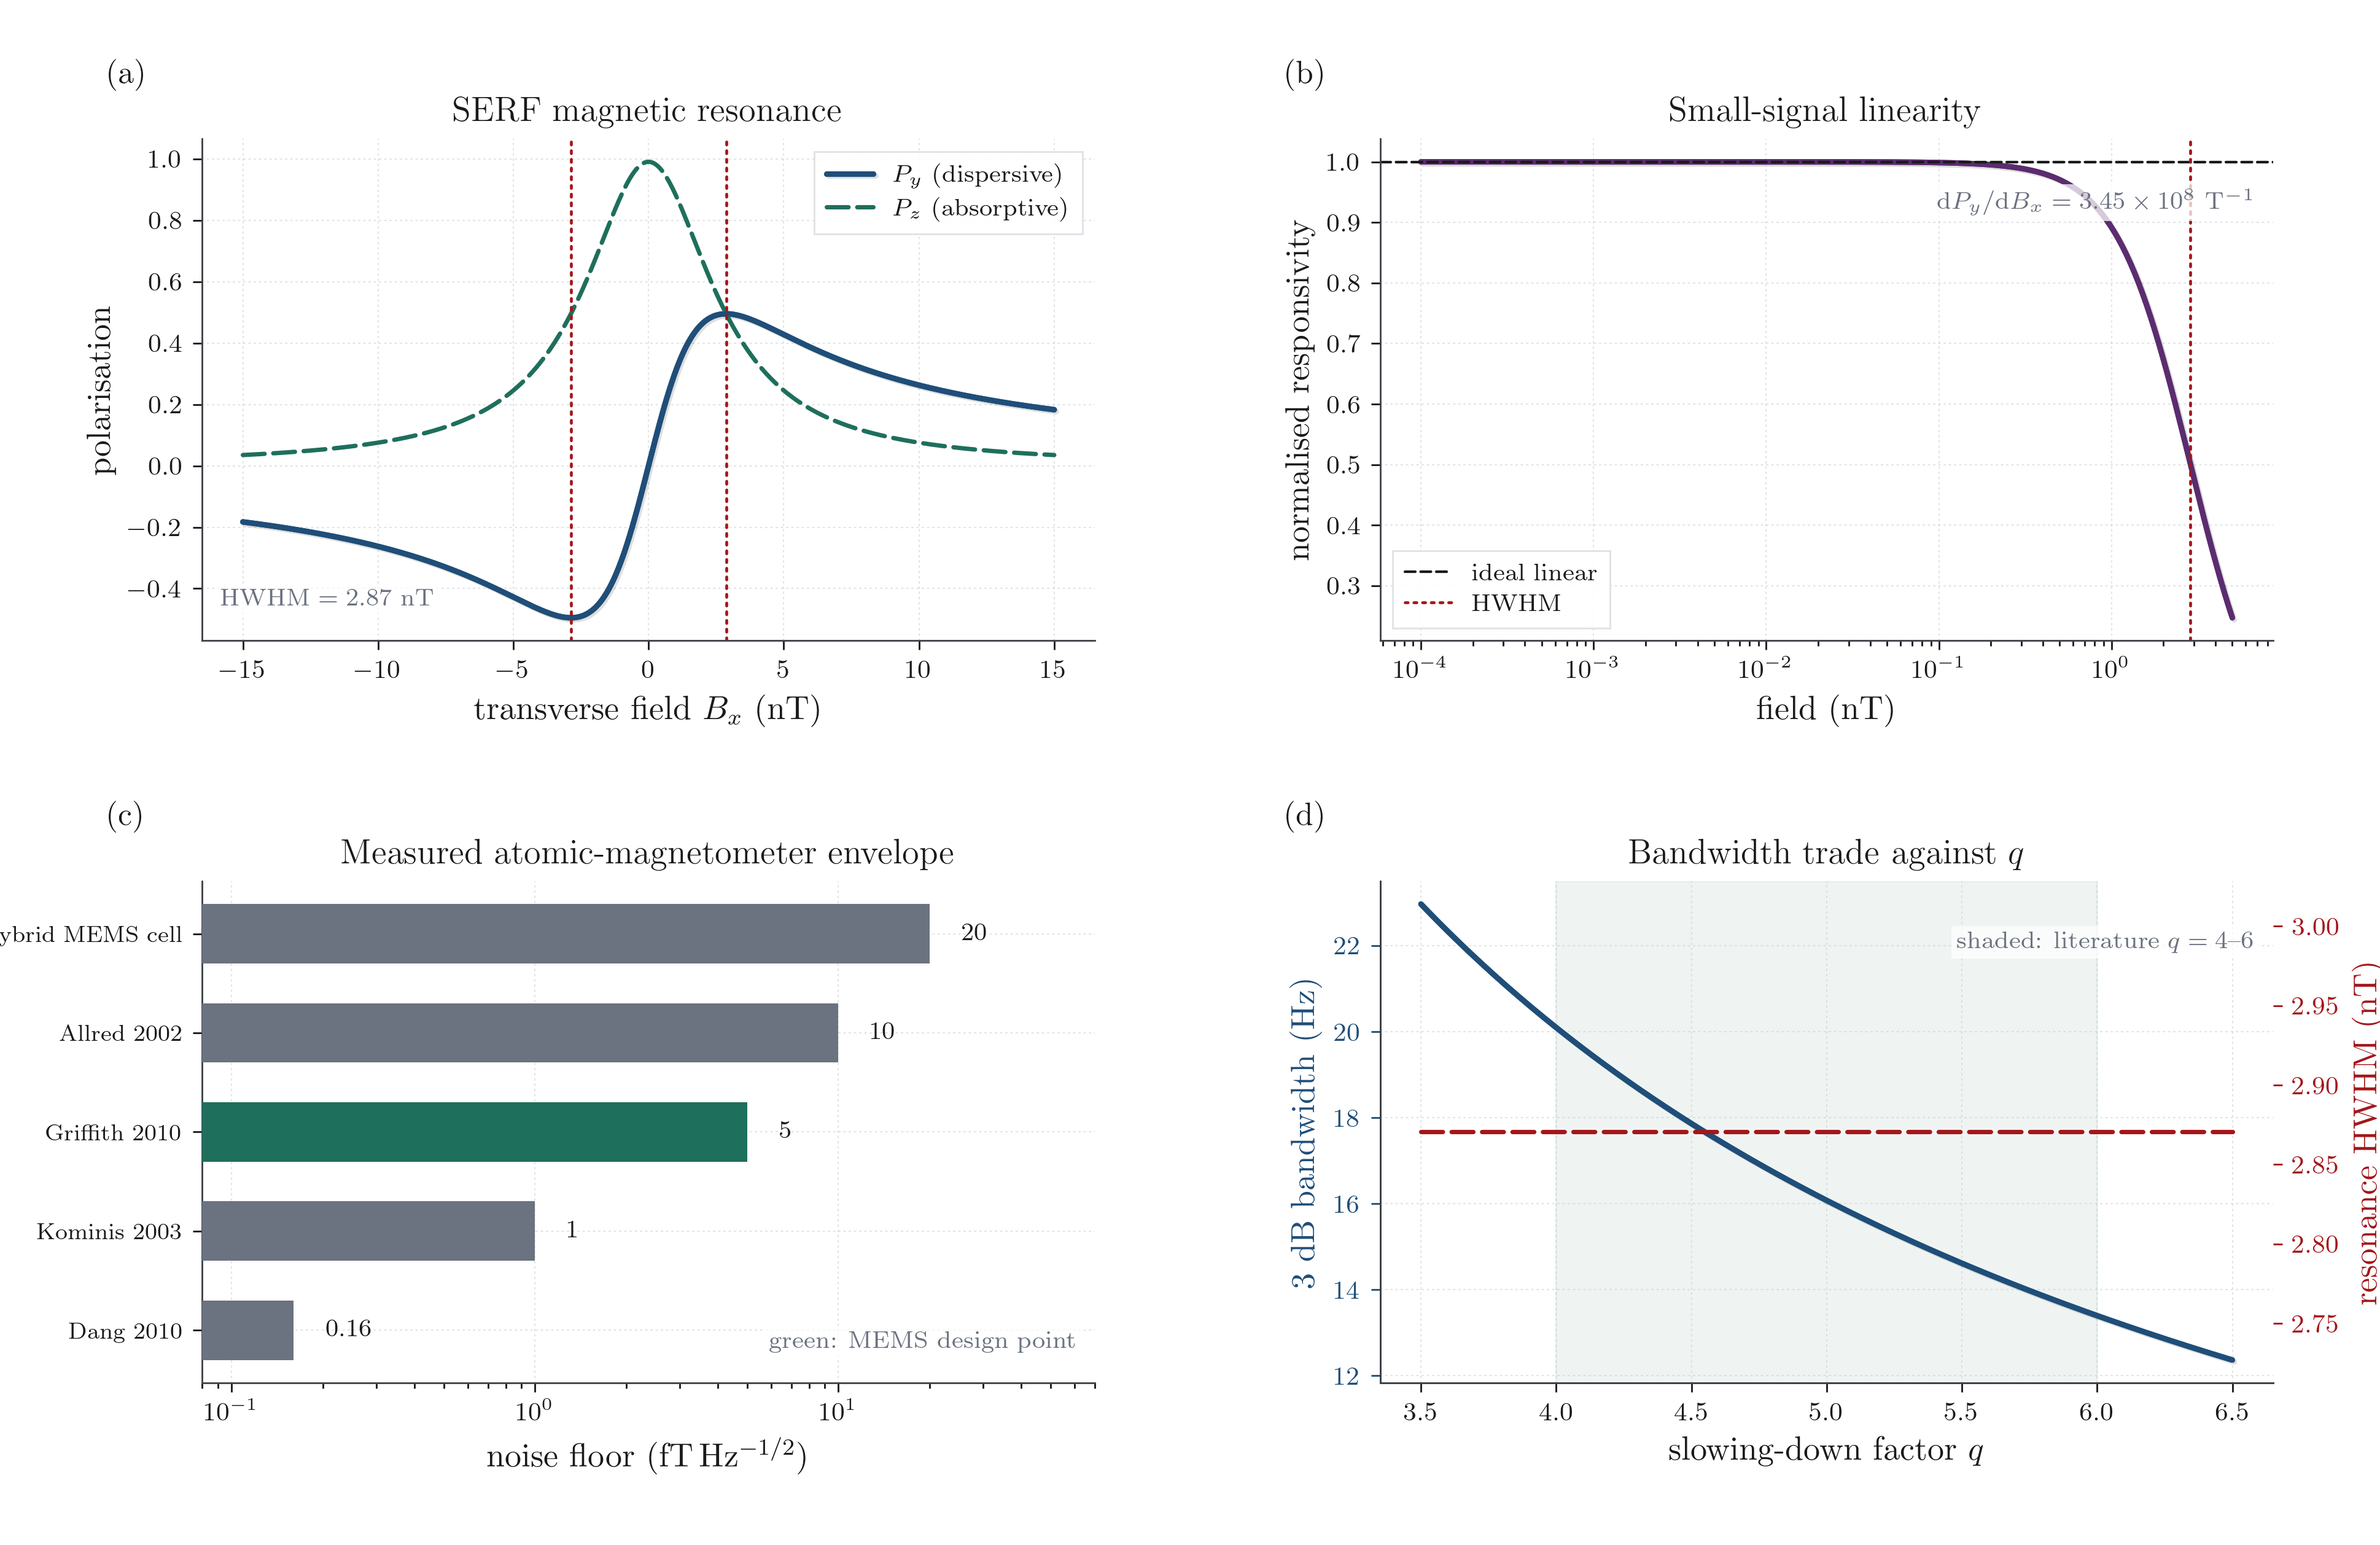
\includegraphics[width=0.72\linewidth]{outputs/fig_sensor_physics.png}
\caption{Sensor physics: resonance lineshape, small-signal linearity, the measured
noise-floor envelope \cite{allred2002,kominis2003,dang2010,griffith2010} with the
MEMS design point highlighted, and the bandwidth trade against slowing-down
factor.}\label{fig:phys}
\end{figure}

\subsection{Ambient-field budget}
Table~\ref{tab:budget} traces the suppression chain across sea states. Attitude
motion converts a static geomagnetic field \cite{ncei} into a body-frame
disturbance of $467\nT$ even in calm water and $7{,}498\nT$ when rough, against a
tolerance of a few nanotesla \cite{borna2022}.

\begin{table}[htbp]\centering\small
\begin{tabular}{lrrrc}
\toprule
\textbf{Sea state}&\textbf{Motion swing}&\textbf{Residual after nulling}&\textbf{CAPE gain}&\textbf{Usable?}\\
\midrule
Calm (SS1)&$467.0\nT$&$4.708\nT$&$0.521$&marginal\\
Moderate (SS3--4)&$2{,}761.7\nT$&$4.742\nT$&$0.518$&marginal\\
Rough (SS5--6)&$7{,}497.5\nT$&$4.804\nT$&$0.513$&marginal\\
\bottomrule
\end{tabular}
\caption{Field budget at $100\times$ passive and $100\times$ active suppression.
The residual meets the nominal window \cite{borna2022} in every sea state, yet
roughly half the gain is lost --- explained in Section~6.3.}\label{tab:budget}
\end{table}

\subsection{The Cross-Axis Projection Error requirement}
This is the report's principal engineering finding. The commonly quoted $\pm5\nT$
figure \cite{borna2022} describes where SERF \emph{operation} persists, not where
SERF \emph{performance} is preserved. Borna \emph{et al.} show that a residual
transverse field tilts the effective sensitive axis and introduces gain and phase
errors \cite{borna2022}; parameterising that tilt as
$\alpha=\arctan(\gamma_eB_{\rm res}/R_{\rm tot})$ scales the on-axis gain by
$\cos\alpha$. At exactly $5\nT$ the tilt is $58.8^{\circ}$ and $48\%$ of the
signal is lost. Requiring no more than $5\%$ loss gives
\begin{equation}
B_{\rm res}\leq\frac{R_{\rm tot}}{\gamma_e}\tan\!\big(\arccos0.95\big)=0.94\nT ,
\label{eq:req}
\end{equation}
a factor $5.3$ tighter than the nominal specification, corresponding to
$5.3\times10^{4}$ ($94$~dB) total suppression rather than $10^{4}$ ($80$~dB). For
$1\%$ loss the requirement tightens to $0.41\nT$. Equation~\eqref{eq:req} is the
single most important design constraint in this report and drives most of
Section~8. Comparable conclusions --- that dynamic cross-axis compensation is
required rather than optional --- have been reached independently for wearable
OPM arrays subject to subject motion \cite{borna2022b,boto2018}.

\begin{figure}[htbp]\centering
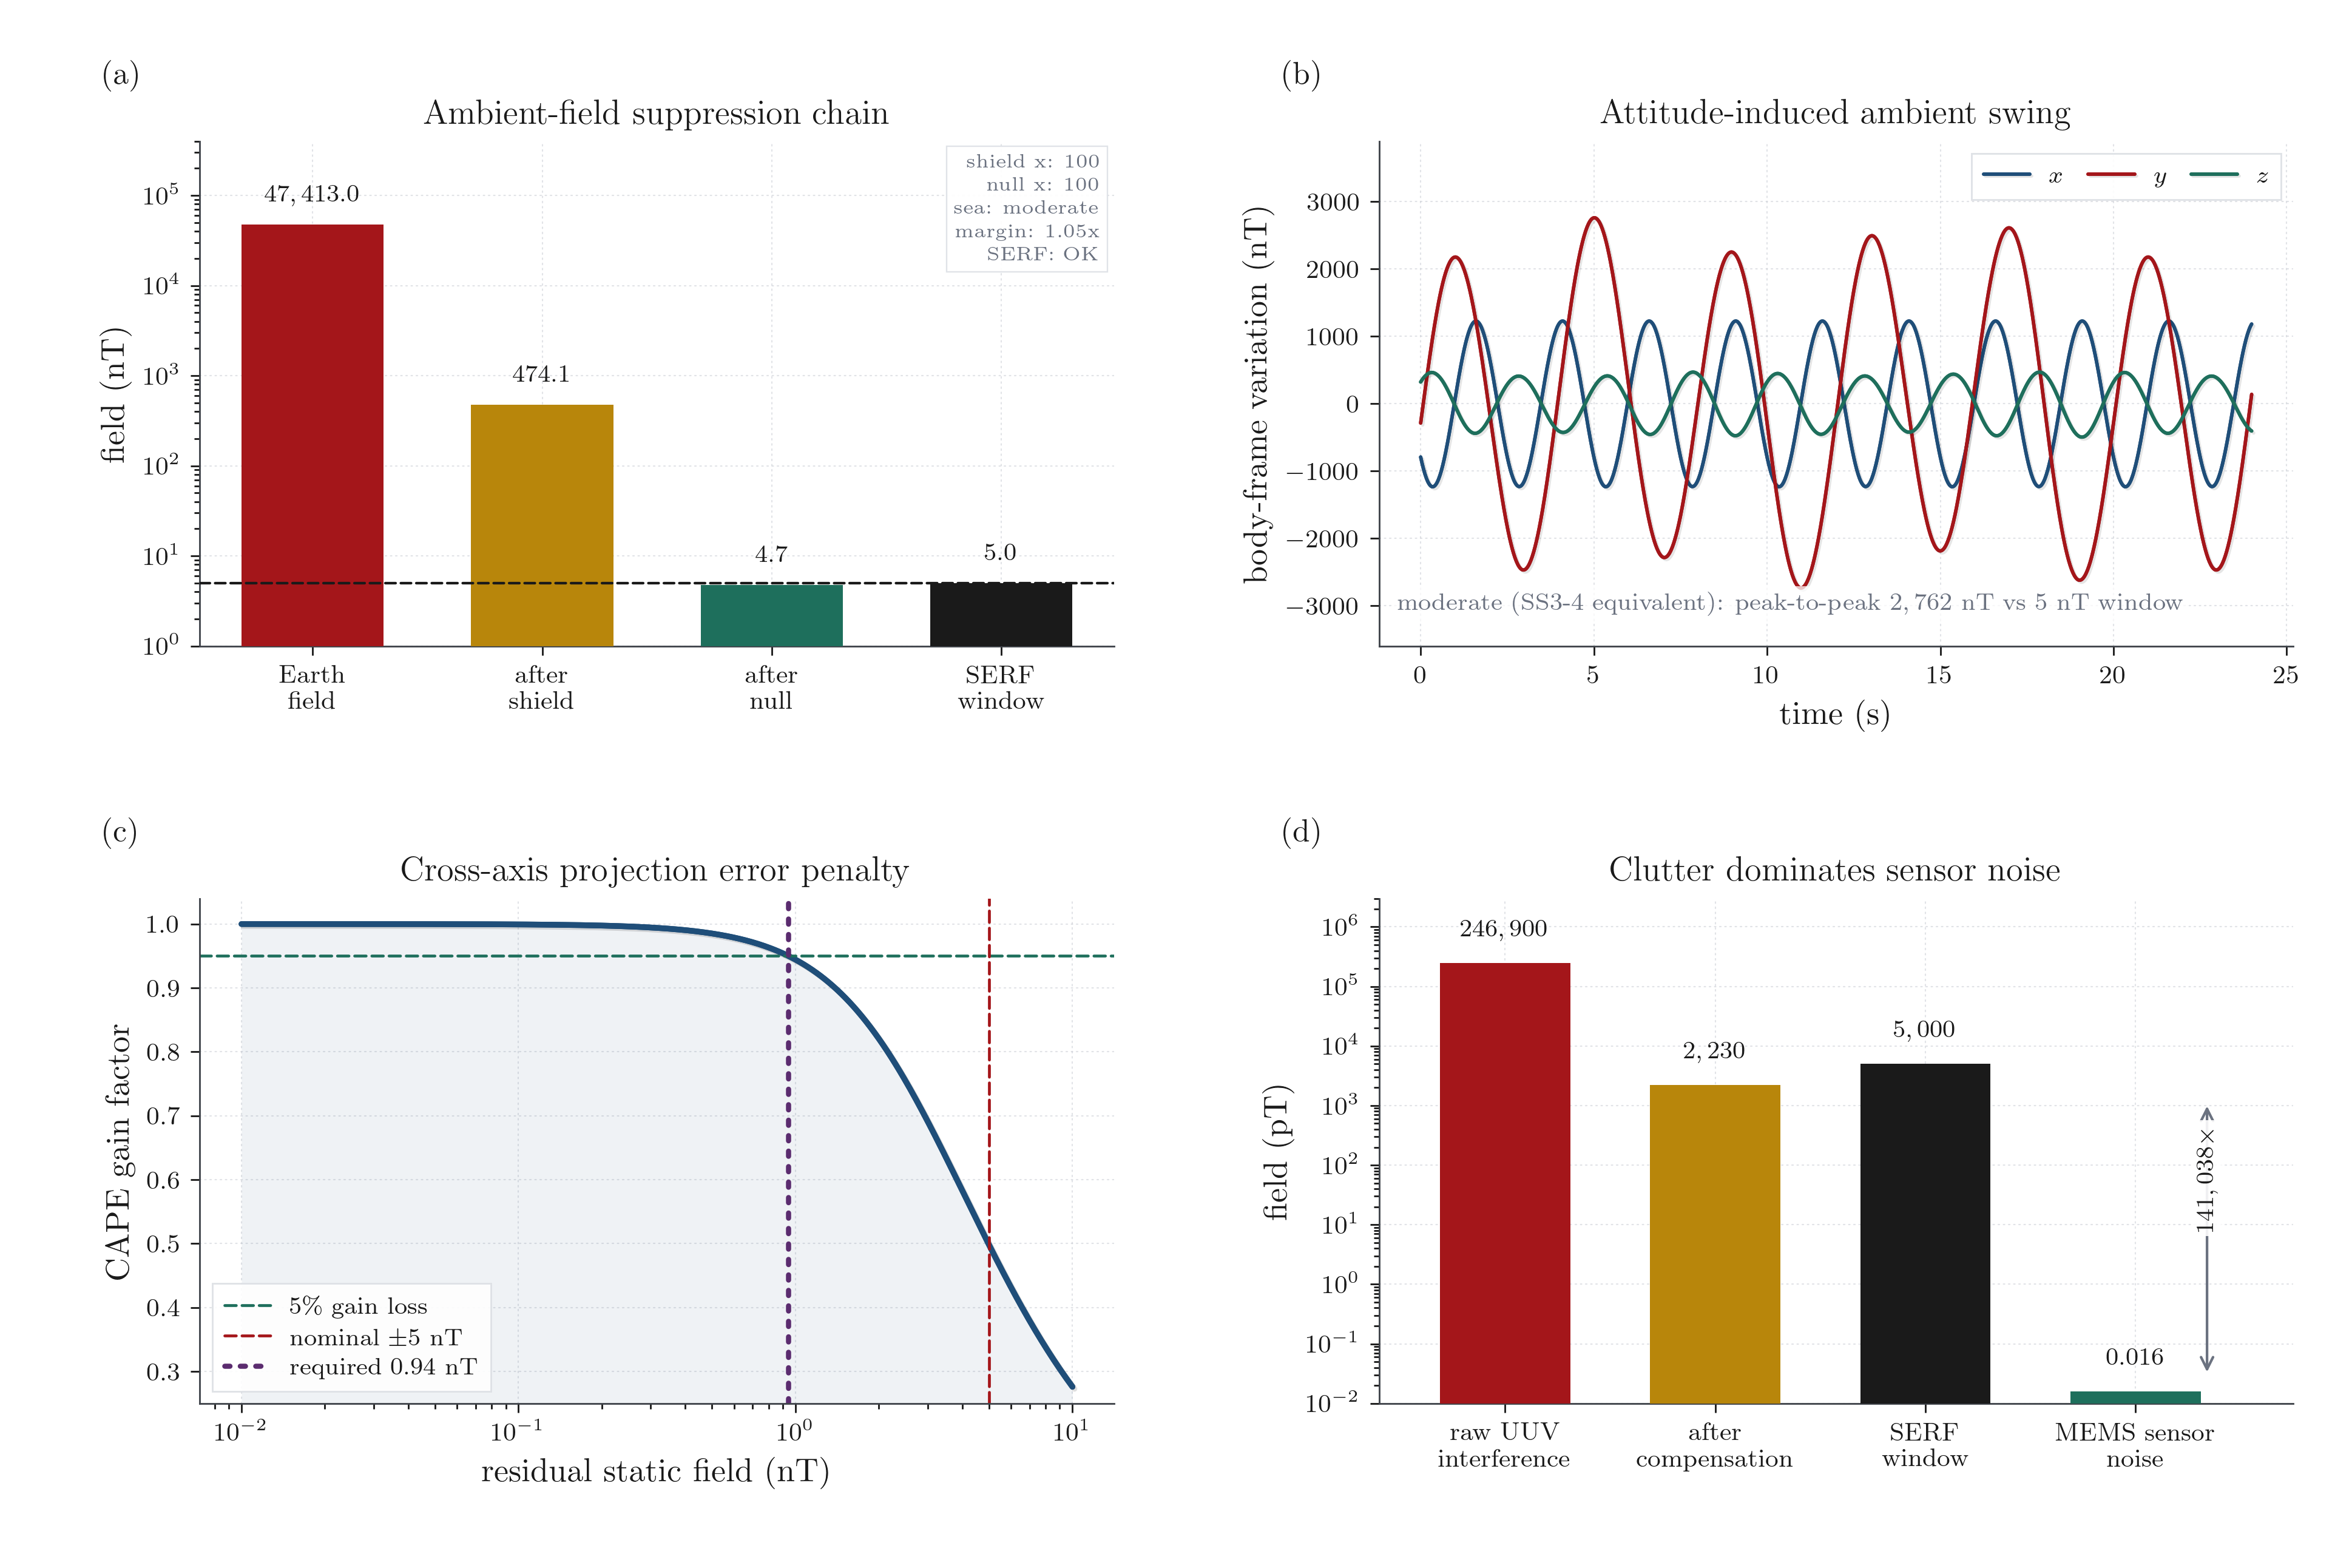
\includegraphics[width=0.74\linewidth]{outputs/fig_field_budget.png}
\caption{Suppression chain, attitude-induced body-frame swing, the CAPE gain
penalty \cite{borna2022} with the derived $0.94\nT$ requirement, and the clutter
hierarchy showing sensor noise \cite{griffith2010} five orders below the
interference residual \cite{oehler2024}.}\label{fig:budget}
\end{figure}

\subsection{Clutter-limited operation}
A $5\fT/\sqrt{\rm Hz}$ cell \cite{griffith2010} in a $10$~Hz band has a noise
floor of $0.016\pT$, against a measured post-compensation vehicle residual of
$2{,}230\pT$ \cite{oehler2024} --- a ratio of $1.4\times10^{5}$
(Figure~\ref{fig:budget}, lower right). The sensitivity analysis confirms the
operational consequence: sensor noise has zero measured influence on detection
range, while clutter magnitude, rejection ratio and gradiometer baseline all
matter. \emph{Procuring a better magnetometer would change nothing.} Effort
belongs on vehicle magnetic cleanliness and processing, which is consistent with
the emphasis of the marine survey literature \cite{oehler2024,seidel2023} and of
aeromagnetic practice \cite{gnadt2022,leliak1961}.

\subsection{Detection performance}
\begin{table}[htbp]\centering\small
\begin{tabular}{lrrl}
\toprule
\textbf{Target class}&\textbf{Moment (A$\cdot$m$^2$)}&\textbf{$R_{50}$ (m)}&\textbf{Basis of moment}\\
\midrule
Micro-UUV, low signature&$5$&$22.3$&engineering estimate\\
Small UXO / ordnance cluster&$50$&$40.7$&engineering estimate\\
Large UXO / naval mine&$500$&$67.6$&scaled from \cite{seidel2023,oehler2024}\\
Submarine, degaussed&$5\times10^{5}$&$267.3$&published moment range \cite{holmes2006}\\
Submarine, undegaussed&$1\times10^{7}$&$503.5$&published moment \cite{holmes2006}\\
\bottomrule
\end{tabular}
\caption{Detection range at $P_{fa}=10^{-4}$, marginalised over target
orientation. The two smallest moments are engineering estimates and are treated
as requirements-driving hypotheticals rather than measured data.}\label{tab:R50}
\end{table}

\begin{figure}[htbp]\centering
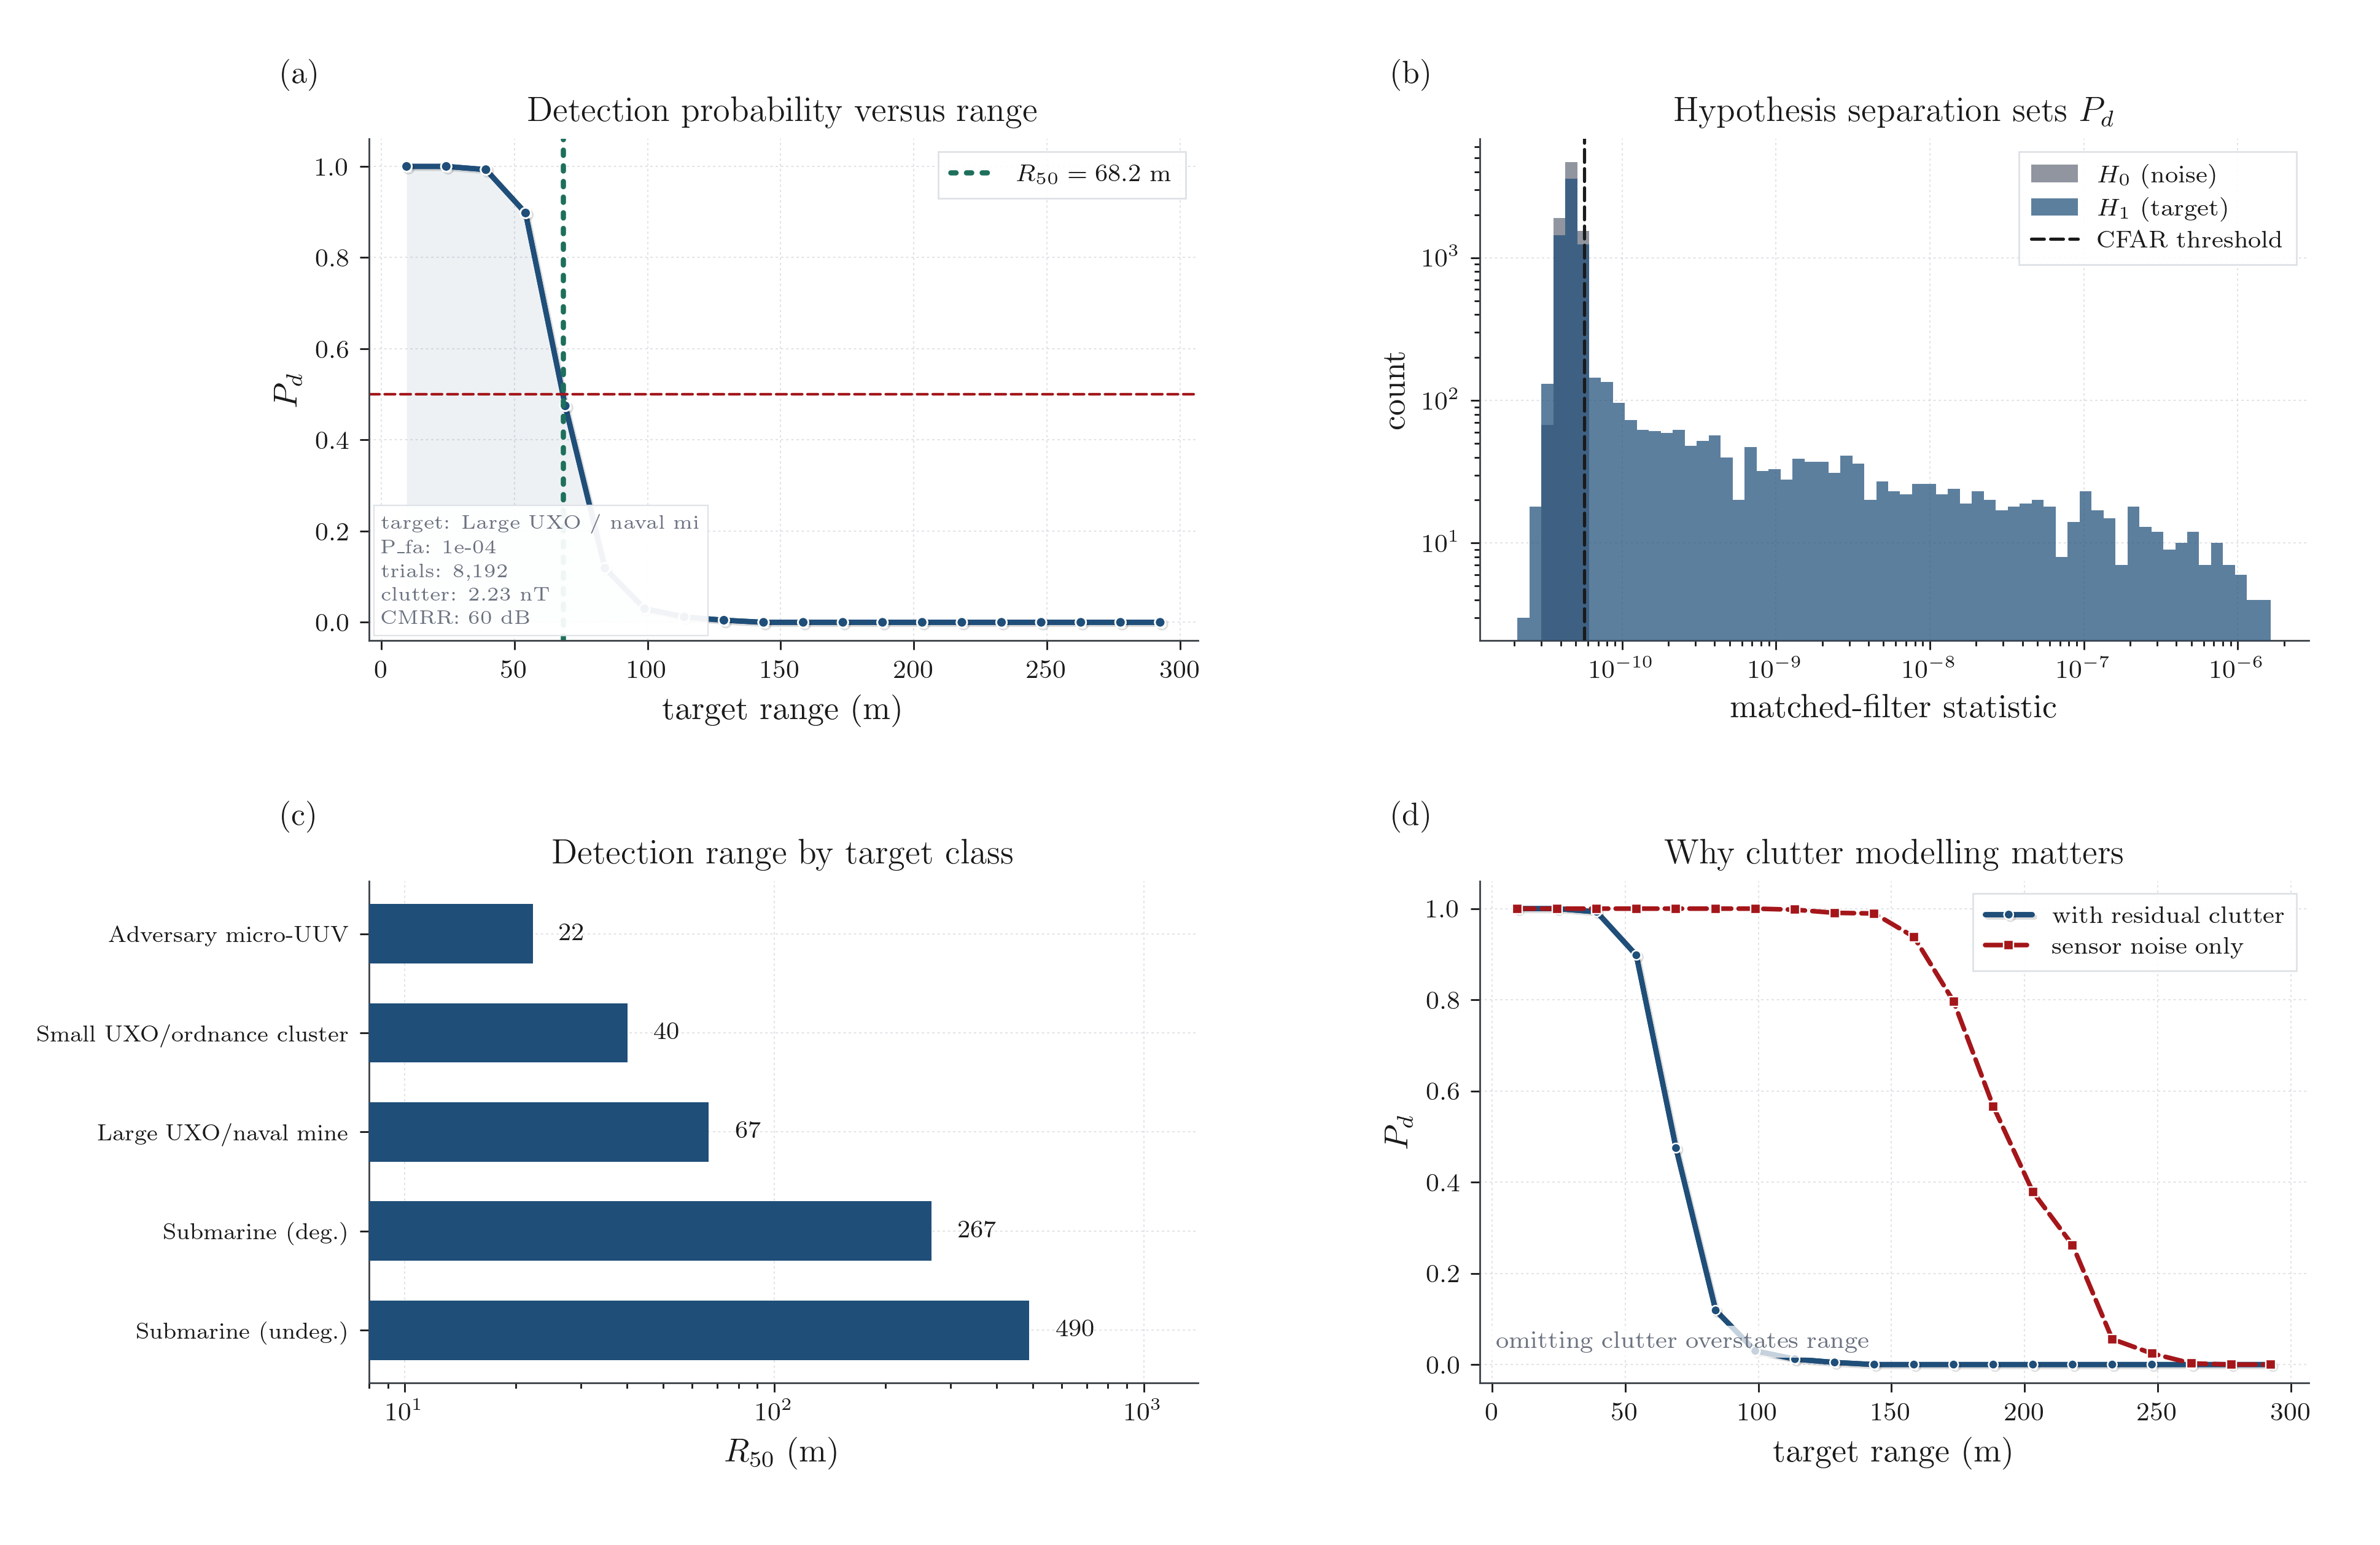
\includegraphics[width=0.70\linewidth]{outputs/fig_detection.png}
\caption{Detection performance: $P_d$ versus range, hypothesis-statistic
separation \cite{vantrees2001}, range by target class, and the effect of
including realistic clutter \cite{oehler2024}.}\label{fig:det}
\end{figure}

Figure~\ref{fig:mission} shows a single transit. Platform clutter exceeds the
target signature by $43\times$ before processing; after compensation and matched
filtering the target is declared at $t=30.01$~s against a true closest approach
of $29.99$~s.

\begin{figure}[htbp]\centering
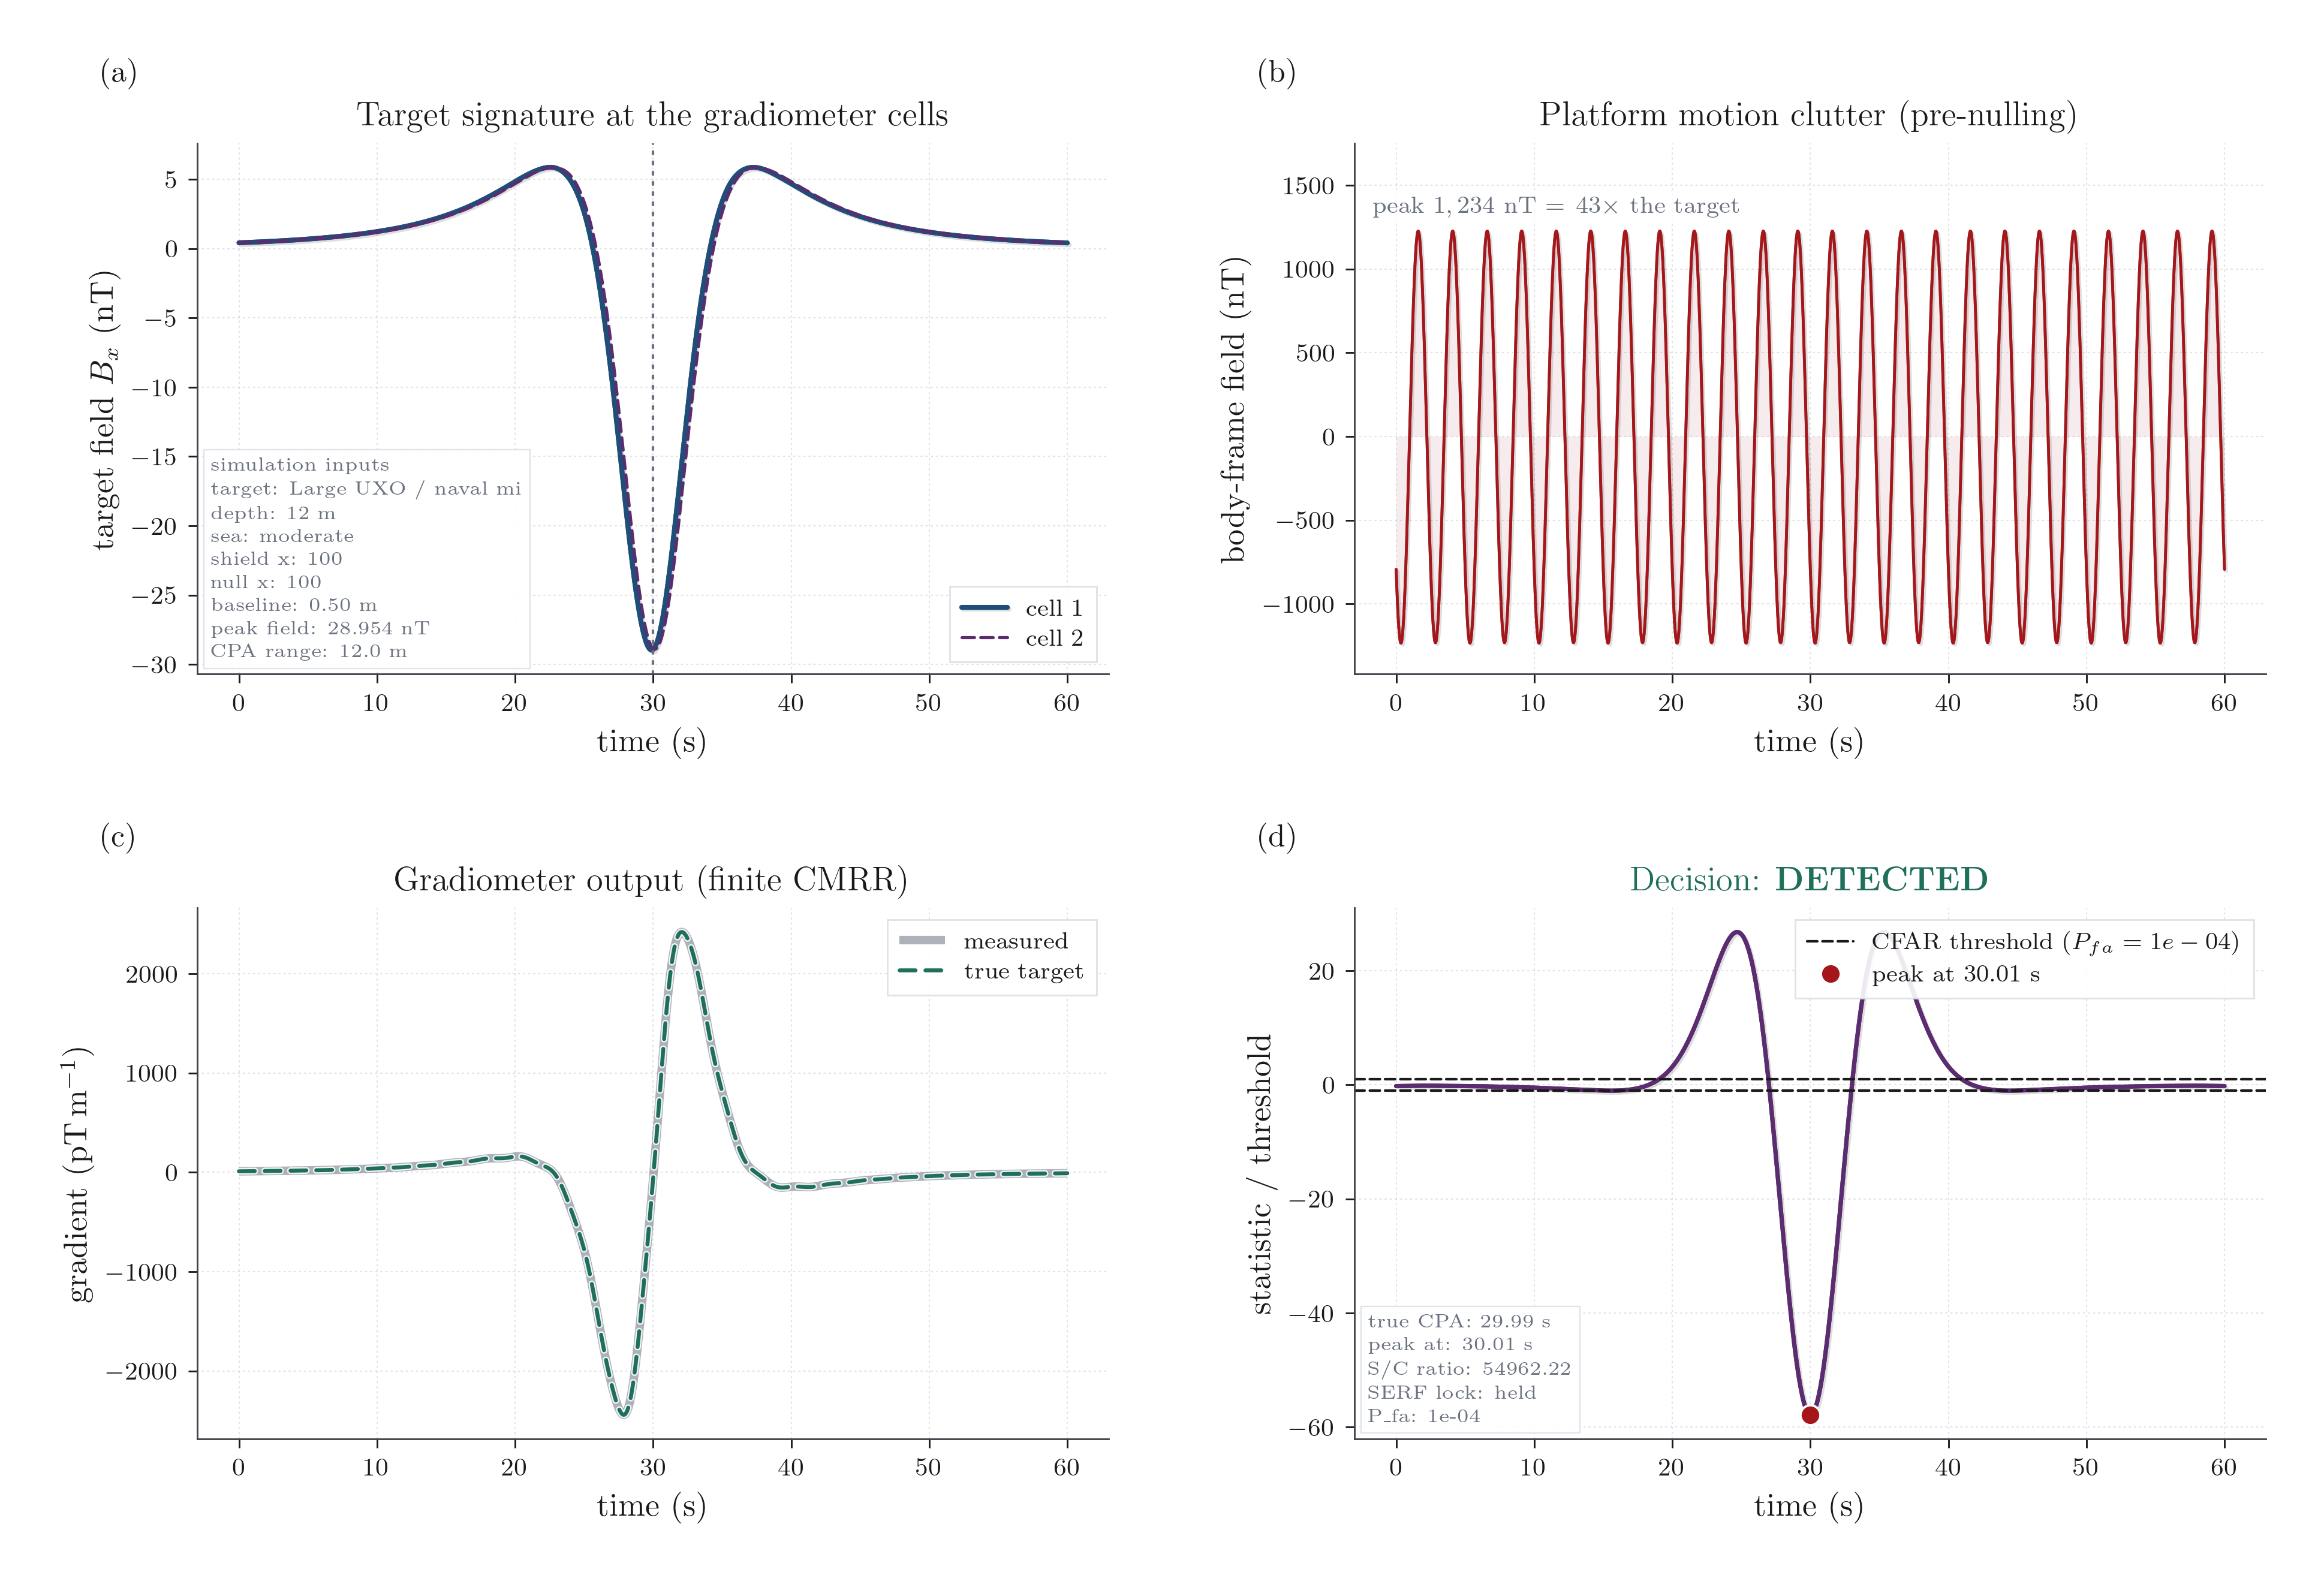
\includegraphics[width=0.68\linewidth]{outputs/fig_mission.png}
\caption{Single transit against a naval-mine-class target at $12$~m standoff.}
\label{fig:mission}
\end{figure}

\section{Discussion}
The concept survives scrutiny, but the engineering emphasis it implies is
counter-intuitive. A programme structured around sensor performance would spend
its budget in the one place the analysis shows to be irrelevant. The binding
constraints are magnetic hygiene and field control --- the same conclusion the
aeromagnetic community reached for aircraft \cite{tolles1950,leliak1961,gnadt2022}
and the marine survey community for AUVs \cite{oehler2024,seidel2023}.

The CAPE result also carries a procurement consequence. A specification written as
``residual field within the SERF window'' would be satisfied by hardware that
nonetheless loses half its sensitivity \cite{borna2022}. Any specification derived
from this work must state Eq.~\eqref{eq:req} together with its gain-loss criterion.

Detection ranges should be read as relative capability across target classes, and
as evidence that the modelling chain yields physically consistent scaling.
Absolute figures inherit the uncertainty of the assumed dipole moments --- two of
which are explicitly estimates --- and of the assumed rejection ratio and clutter
spectrum.

\section{Component Requirements}
The following requirements follow from the analysis; each is traceable to a
specific result or source rather than asserted.

\begin{table}[H]\centering\scriptsize
\begin{tabular}{p{0.8cm}p{2.5cm}p{6.6cm}p{4.5cm}}
\toprule
\textbf{Req}&\textbf{Subsystem}&\textbf{Requirement}&\textbf{Derivation}\\
\midrule
R-01&Field control&Residual static field at cell $\leq0.94\nT$; goal $0.41\nT$&Eq.~\eqref{eq:req}; CAPE \cite{borna2022}\\
R-02&Shield + coils&Combined suppression $\geq94$~dB from $50{,}000\nT$ ambient&R-01 with \cite{ncei}\\
R-03&Nulling servo&Closed-loop bandwidth $\geq10\times$ wave encounter frequency ($\geq5$~Hz for $0.5$~Hz seas); slew $\geq8{,}000\nT$/s&Rough-sea swing (Table~\ref{tab:budget}); cf.\ \cite{fang2012,borna2022b}\\
R-04&Reference magnetometer&Noise floor $\leq0.1\nT$ in band; three-axis; bandwidth $\geq$ servo bandwidth&Servo cannot null below its reference \cite{seltzer2004}\\
R-05&Coil driver&Current noise contributing $\leq0.1\nT$ at the cell; DAC resolution $\geq18$~bit over $\pm60{,}000\nT$ full scale&$6\times10^{5}$ levels $\Rightarrow2^{18}$; shield noise floor \cite{lee2008}\\
R-06&Vapour cell&MEMS, hermetic anodic bond, $\geq1$~mm$^3$; survive shock and vibration without buffer-gas loss&\cite{griffith2010,liew2004}\\
R-07&Cell heater&$150$--$200^{\circ}$C, stability $\pm5$~mK, non-magnetic (AC or counter-wound) drive&Density sets sensitivity \cite{allred2002,fang2015}\\
R-08&Laser&Pump and probe at the alkali D1 line ($\approx795$~nm for Rb); frequency stability $\leq1$~MHz; probe broadening below spin-destruction rate&\cite{griffith2010,shah2009}\\
R-09&Gradiometer&Two cells, baseline $\geq0.5$~m, common-mode rejection $\geq60$~dB, gain and axis matching $\leq0.1\%$&Elasticity test S-4; \cite{oehler2024}\\
R-10&Platform magnetics&Post-compensation residual $\leq2.23\nT$; non-magnetic fasteners, thruster shielding, DC current-loop minimisation&\cite{oehler2024}; clutter dominates (S-4)\\
R-11&Attitude sensing&IMU delivering roll/pitch/yaw to $\leq0.05^{\circ}$, synchronised to the magnetometer within $1$~ms&Tolles--Lawson fit quality \cite{tolles1950,gnadt2022,leliak1961}\\
R-12&Signal chain&$\geq24$-bit ADC, $\geq100$~Hz sampling, anti-alias filtered below sensor bandwidth ($\approx16$~Hz)&Sensor 3~dB bandwidth (Fig.~\ref{fig:phys})\\
R-13&Sensor placement&Boom or tow displacement maximising distance from thrusters and battery&Clutter falls as $r^{-3}$ \cite{jackson1998,oehler2024}\\
\bottomrule
\end{tabular}
\caption{Component requirements derived from the simulation.}\label{tab:req}
\end{table}

Two requirements interact and deserve emphasis. R-03 and R-04 together define the
hardest single component: a reference magnetometer that is simultaneously
low-noise, three-axis, wide-band, and physically close to the SERF cell without
magnetically contaminating it. R-02 and R-10 compete for the same volume, since
shielding material added near the cell is itself a potential magnetic source and
contributes its own Johnson-current noise \cite{lee2008}.

\section{Limitations, Challenges and Barriers}
\subsection{Modelling limitations}
\begin{enumerate}[leftmargin=1.5em]
\item \textbf{No absolute sensitivity prediction.} The model carries no atom
number, cell volume or photon shot-noise term \cite{allred2002,mitchell2020}, so
it cannot independently predict a $\fT/\sqrt{\rm Hz}$ figure; published values
\cite{griffith2010} are adopted and checked for consistency. Closing this gap is
the highest-value next step.
\item \textbf{Platform self-field is parametric.} Vehicle interference is
represented by a rejection ratio and a $1/f$ residual rather than derived from
hull geometry and materials, so R-09 and R-10 rest on a published benchmark
\cite{oehler2024} rather than a model of the specific vehicle.
\item \textbf{Quasi-static nulling.} The field budget evaluates suppression at the
dominant motion frequency and does not simulate closed-loop servo dynamics
\cite{fang2012}, so it cannot yet predict loss of SERF lock during a transient
manoeuvre.
\item \textbf{Two target moments are estimates.} The micro-UUV and small-UXO
moments are requirements-driving hypotheticals; ranges for those classes should
not be quoted as capability.
\item \textbf{Single-species, single-cell treatment.} Hybrid pumping
\cite{ito2016}, cell-to-cell variation and multi-species effects are not modelled.
\item \textbf{Ensemble-averaged spin.} Valid at operating densities
\cite{seltzer2008}, but excludes spin-squeezing approaches that could raise the
sensitivity ceiling \cite{mitchell2020}.
\end{enumerate}

\subsection{Engineering and programmatic barriers}
\begin{enumerate}[leftmargin=1.5em]
\item \textbf{Dynamic range is the fundamental tension.} The sensor must resolve
picotesla while immersed in a field $10^{7}$ times larger \cite{ncei} that swings
by thousands of nanotesla with the sea, and every subsystem inherits this. A
nulling failure does not degrade gracefully --- the sensor leaves the SERF regime
and stops working \cite{allred2002,borna2022}. Mitigation requires sustained servo
authority or a designed fallback mode (e.g.\ scalar operation \cite{shah2007}),
and no such fallback exists here.
\item \textbf{Thermal budget versus vehicle power.} Holding $150$--$200^{\circ}$C
at $\pm5$~mK in cold seawater using non-magnetic heating
\cite{fang2015,griffith2010} is a continuous draw on an endurance-limited
platform, and heater currents are themselves a magnetic risk.
\item \textbf{Magnetic hygiene is a whole-vehicle constraint.} R-10 applies to the
AUV, not the payload. Thrusters, battery current loops and steel fasteners must be
controlled at design time \cite{oehler2024}; retrofitting a SERF payload to an
existing vehicle is likely to fail on this basis alone.
\item \textbf{Shock and vibration unproven at system level.} The MEMS cell is
robust \cite{liew2004,griffith2010}, but the optical bench, fibre alignment and
coil formers must survive launch and recovery while holding the alignment
tolerances of R-09.
\item \textbf{Short detection ranges against small targets.} At $22$--$68$~m, area
coverage rate is low and mission planning becomes demanding. For mine
countermeasures this may be acceptable \cite{seidel2023}; for wide-area search it
may not, and that trade should be settled before investment.
\item \textbf{Heading dependence.} Any residual field couples through CAPE
\cite{borna2022}, so sensor gain may vary with vehicle heading, appearing
operationally as a direction-dependent detection range. Heading error is a known
issue in atomic magnetometry \cite{seltzer2008,alexandrov1995} and demands in-situ
calibration.
\item \textbf{Field calibration and drift.} Although the atomic transition is
intrinsically calibrated \cite{budker2007}, the surrounding chain --- coil
constants, axis alignment, compensation coefficients --- is not. Compensation
manoeuvres are needed to condition the Tolles--Lawson fit
\cite{leliak1961,leach1980}, and these consume mission time.
\item \textbf{Validation data availability.} Compensation performance rests on a
single published UUV benchmark \cite{oehler2024}; independent replication on the
target vehicle is needed before performance claims are made.
\item \textbf{Technology readiness.} The individual pieces are demonstrated
\cite{griffith2010,oehler2024,fang2012}; an integrated, ruggedised,
vehicle-mounted SERF gradiometer with active nulling is not. Treat as TRL~3--4,
with integration risk concentrated in the nulling servo.
\end{enumerate}

\subsection{Conditions under which the concept fails}
It is worth being explicit. The concept does not close if any of the following
proves true: sustained $94$~dB suppression cannot be maintained through vehicle
manoeuvres; vehicle magnetic residual cannot be reduced to the few-nanotesla class
on the target platform \cite{oehler2024}; the thermal budget is incompatible with
mission endurance; or operational requirements demand detection ranges against
low-signature targets substantially beyond Table~\ref{tab:R50}. Each is testable
early and cheaply relative to full development, and the recommended programme
structure is to test them first.

\section{Recommendations and Next Steps}
\begin{enumerate}[leftmargin=1.5em]
\item Extend the sensor model with atom number and photon shot noise
\cite{allred2002,mitchell2020} to enable absolute sensitivity prediction and
closure against published devices \cite{griffith2010}.
\item Implement closed-loop nulling with explicit servo dynamics
\cite{fang2012,borna2022b} and simulate loss of SERF lock under transient
manoeuvres --- the principal unmodelled failure mode.
\item Replace the parametric rejection ratio with a geometry-based vehicle
magnetic model \cite{tolles1950,gnadt2022} for the specific target platform.
\item Bench-validate CAPE using a shielded MEMS cell on a rotation stage; this
directly tests Eq.~\eqref{eq:req}, the report's central claim, at modest cost,
following the experimental approach of \cite{borna2022}.
\item Extend GPU validation beyond the single Ampere-class device verified here
to the multi-GPU and non-Ampere configurations a deployed processing chain would
plausibly use.
\item Obtain measured signature data for the small-target classes to replace the
two engineering estimates.
\item Conduct an early magnetic survey of the candidate AUV \cite{oehler2024} to
establish whether R-10 is achievable before further investment.
\end{enumerate}

\section{Conclusion}
A ruggedised SERF MEMS magnetometer is a physically credible AUV MAD payload. Its
feasibility is governed not by sensor sensitivity, which exceeds requirement by
five orders of magnitude \cite{griffith2010,oehler2024}, but by ambient-field
control and platform magnetic cleanliness. The nominal SERF field window
\cite{borna2022} is shown to be insufficient by a factor of $5.3$ once the
Cross-Axis Projection Error is accounted for, giving a $94$~dB suppression
requirement that drives the majority of the component specification. All
twenty-seven verification, validation and stress tests pass, including agreement
between an independent quantum reference model \cite{qutip2013} and the production
solver \cite{seltzer2008} to $2.8\times10^{-16}$, and an emergent range-law
exponent of $0.244$ against a predicted $0.25$ \cite{jackson1998}. The barriers to
implementation are identified and concentrated in the nulling servo and
whole-vehicle magnetic design; each is testable early, and testing them first is
the recommended programme structure.

\begin{thebibliography}{99}\small
\bibitem{allred2002} J.~C.~Allred, R.~N.~Lyman, T.~W.~Kornack, and M.~V.~Romalis,
``High-sensitivity atomic magnetometer unaffected by spin-exchange relaxation,''
\emph{Phys. Rev. Lett.} \textbf{89}(13), 130801 (2002).
DOI:10.1103/PhysRevLett.89.130801.

\bibitem{kominis2003} I.~K.~Kominis, T.~W.~Kornack, J.~C.~Allred, and
M.~V.~Romalis, ``A subfemtotesla multichannel atomic magnetometer,''
\emph{Nature} \textbf{422}(6932), 596--599 (2003). DOI:10.1038/nature01484.

\bibitem{dang2010} H.~B.~Dang, A.~C.~Maloof, and M.~V.~Romalis, ``Ultrahigh
sensitivity magnetic field and magnetization measurements with an atomic
magnetometer,'' \emph{Appl. Phys. Lett.} \textbf{97}(15), 151110 (2010).
DOI:10.1063/1.3491215.

\bibitem{griffith2010} W.~C.~Griffith, S.~Knappe, and J.~Kitching, ``Femtotesla
atomic magnetometry in a microfabricated vapor cell,'' \emph{Opt. Express}
\textbf{18}(26), 27167--27172 (2010). DOI:10.1364/OE.18.027167.

\bibitem{shah2007} V.~Shah, S.~Knappe, P.~D.~D.~Schwindt, and J.~Kitching,
``Subpicotesla atomic magnetometry with a microfabricated vapour cell,''
\emph{Nature Photonics} \textbf{1}(11), 649--652 (2007).
DOI:10.1038/nphoton.2007.201.

\bibitem{borna2022} A.~Borna, J.~Iivanainen, T.~R.~Carter, J.~McKay, S.~Taulu,
J.~Stephen, and P.~D.~D.~Schwindt, ``Cross-axis projection error in optically
pumped magnetometers and its implication for magnetoencephalography systems,''
\emph{NeuroImage} \textbf{247}, 118818 (2022).
DOI:10.1016/j.neuroimage.2021.118818.

\bibitem{borna2022b} A.~Borna \emph{et al.}, ``Cross-axis dynamic field
compensation of optically pumped magnetometer arrays for MEG,''
\emph{NeuroImage} \textbf{262}, 119559 (2022).
DOI:10.1016/j.neuroimage.2022.119559.

\bibitem{seltzer2008} S.~J.~Seltzer, \emph{Developments in Alkali-Metal Atomic
Magnetometry}, Ph.D. dissertation, Department of Physics, Princeton University
(2008).

\bibitem{savukov2005} I.~M.~Savukov and M.~V.~Romalis, ``Effects of spin-exchange
collisions in a high-density alkali-metal vapor in low magnetic fields,''
\emph{Phys. Rev. A} \textbf{71}, 023405 (2005). DOI:10.1103/PhysRevA.71.023405.

\bibitem{budker2007} D.~Budker and M.~V.~Romalis, ``Optical magnetometry,''
\emph{Nature Physics} \textbf{3}(4), 227--234 (2007). DOI:10.1038/nphys566.

\bibitem{li2018} J.~Li, W.~Quan, B.~Zhou, Z.~Wang, J.~Lu, Z.~Hu, G.~Liu, and
J.~Fang, ``SERF atomic magnetometer -- recent advances and applications: a
review,'' \emph{IEEE Sensors Journal} \textbf{18}(20), 8198--8207 (2018).

\bibitem{happer1977} W.~Happer and A.~C.~Tam, ``Effect of rapid spin exchange on
the magnetic-resonance spectrum of alkali vapors,'' \emph{Phys. Rev. A}
\textbf{16}, 1877 (1977).

\bibitem{oehler2024} M.~Oehler \emph{et al.}, ``Processing of unmanned underwater
vehicle vector magnetometer data,'' \emph{Geophysical Prospecting} \textbf{72}
(2024). DOI:10.1111/1365-2478.13556.

\bibitem{seidel2023} M.~Seidel \emph{et al.}, ``Underwater UXO detection using
magnetometry on hovering AUVs,'' \emph{Journal of Applied Geophysics} / BASTA
project reporting (2023).

\bibitem{tolles1950} W.~E.~Tolles and J.~D.~Lawson, ``Magnetic compensation of
MAD equipped aircraft,'' Airborne Instruments Laboratory, Rept. 201-1 (1950).

\bibitem{gnadt2022} A.~R.~Gnadt, A.~B.~Wollaber, and A.~P.~Nielsen, ``Derivation
and extensions of the Tolles-Lawson model for aeromagnetic compensation,''
arXiv:2212.09899 (2022).

\bibitem{leliak1961} P.~Leliak, ``Identification and evaluation of magnetic-field
sources of magnetic airborne detector equipped aircraft,'' \emph{IRE Trans.
Aerospace and Navigational Electronics} \textbf{8}(3), 95--105 (1961).

\bibitem{leach1980} B.~W.~Leach, ``Aeromagnetic compensation as a linear
regression problem,'' in \emph{Information Linkage Between Applied Mathematics
and Industry II}, Academic Press (1980).

\bibitem{jackson1998} J.~D.~Jackson, \emph{Classical Electrodynamics}, 3rd ed.,
Wiley, New York (1998), Ch.~5.

\bibitem{wynn1975} W.~M.~Wynn \emph{et al.}, ``Advanced superconducting
gradiometer/magnetometer arrays and a novel signal processing technique,''
\emph{IEEE Trans. Magnetics} \textbf{11}(2), 701--707 (1975).

\bibitem{vantrees2001} H.~L.~Van~Trees, \emph{Detection, Estimation, and
Modulation Theory, Part I}, Wiley (2001).

\bibitem{kay1998} S.~M.~Kay, \emph{Fundamentals of Statistical Signal Processing,
Vol.~II: Detection Theory}, Prentice Hall (1998).

\bibitem{ncei} National Centers for Environmental Information (NOAA),
``Geomagnetism frequently asked questions,'' and the International Geomagnetic
Reference Field (IGRF-13). Earth field intensity $25{,}000$--$65{,}000\nT$.

\bibitem{lindblad1976} G.~Lindblad, ``On the generators of quantum dynamical
semigroups,'' \emph{Commun. Math. Phys.} \textbf{48}(2), 119--130 (1976).

\bibitem{breuer2002} H.-P.~Breuer and F.~Petruccione, \emph{The Theory of Open
Quantum Systems}, Oxford University Press (2002).

\bibitem{qutip2013} J.~R.~Johansson, P.~D.~Nation, and F.~Nori, ``QuTiP 2: a
Python framework for the dynamics of open quantum systems,'' \emph{Comput. Phys.
Commun.} \textbf{184}, 1234 (2013).

\bibitem{butcher2016} J.~C.~Butcher, \emph{Numerical Methods for Ordinary
Differential Equations}, 3rd ed., Wiley (2016).

\bibitem{diebel2006} J.~Diebel, ``Representing attitude: Euler angles, unit
quaternions, and rotation vectors,'' Stanford University technical report (2006).

\bibitem{marsaglia1972} G.~Marsaglia, ``Choosing a point from the surface of a
sphere,'' \emph{Ann. Math. Statist.} \textbf{43}(2), 645--646 (1972).

\bibitem{oberkampf2010} W.~L.~Oberkampf and C.~J.~Roy, \emph{Verification and
Validation in Scientific Computing}, Cambridge University Press (2010).

\bibitem{lee2008} S.-K.~Lee and M.~V.~Romalis, ``Calculation of magnetic field
noise from high-permeability magnetic shields and conducting objects with simple
geometry,'' \emph{J. Appl. Phys.} \textbf{103}(8), 084904 (2008).

\bibitem{liew2004} L.-A.~Liew, S.~Knappe, J.~Moreland, H.~Robinson, L.~Hollberg,
and J.~Kitching, ``Microfabricated alkali atom vapor cells,'' \emph{Appl. Phys.
Lett.} \textbf{84}(14), 2694--2696 (2004).

\bibitem{schwindt2004} P.~D.~D.~Schwindt, S.~Knappe, V.~Shah, L.~Hollberg,
J.~Kitching, L.-A.~Liew, and J.~Moreland, ``Chip-scale atomic magnetometer,''
\emph{Appl. Phys. Lett.} \textbf{85}(26), 6409--6411 (2004).

\bibitem{seltzer2004} S.~J.~Seltzer and M.~V.~Romalis, ``Unshielded three-axis
vector operation of a spin-exchange-relaxation-free atomic magnetometer,''
\emph{Appl. Phys. Lett.} \textbf{85}(20), 4804--4806 (2004).

\bibitem{fang2012} J.~Fang and J.~Qin, ``In situ triaxial magnetic field
compensation for the spin-exchange-relaxation-free atomic magnetometer,''
\emph{Rev. Sci. Instrum.} \textbf{83}(10), 103104 (2012).

\bibitem{fang2015} J.~Fang, R.~Li, L.~Duan, Y.~Chen, and W.~Quan, ``Study of the
operation temperature in the spin-exchange relaxation free magnetometer,''
\emph{Rev. Sci. Instrum.} \textbf{86}, 073116 (2015).

\bibitem{shah2009} V.~Shah and M.~V.~Romalis, ``Spin-exchange relaxation-free
magnetometry using elliptically polarized light,'' \emph{Phys. Rev. A}
\textbf{80}, 013416 (2009).

\bibitem{wei2023} K.~Wei, T.~Zhao, X.~Fang, \emph{et al.}, ``The suppression of
the probe laser pumping effect in SERF atomic magnetometer,'' \emph{Frontiers in
Physics} \textbf{11}, 1181399 (2023).

\bibitem{boto2018} E.~Boto \emph{et al.}, ``Moving magnetoencephalography towards
real-world applications with a wearable system,'' \emph{Nature} \textbf{555}(7698),
657--661 (2018).

\bibitem{mitchell2020} M.~W.~Mitchell and S.~Palacios~Alvarez, ``Colloquium:
Quantum limits to the energy resolution of magnetic field sensors,'' \emph{Rev.
Mod. Phys.} \textbf{92}, 021001 (2020).

\bibitem{ito2016} Y.~Ito, D.~Sato, K.~Kamada, and T.~Kobayashi, ``Optimal
densities of alkali metal atoms in an optically pumped K-Rb hybrid atomic
magnetometer,'' \emph{Opt. Express} \textbf{24}(14), 15391 (2016).

\bibitem{alexandrov1995} E.~B.~Alexandrov \emph{et al.}, ``Laser pumping in the
scheme of an Mx-magnetometer,'' \emph{Optics and Spectroscopy} \textbf{78}, 292
(1995).

\bibitem{clem1997} T.~R.~Clem, ``Superconducting magnetic sensors for mine
detection and classification,'' Naval Surface Warfare Center, Coastal Systems
Station, Panama City (1997).

\bibitem{holmes2006} J.~J.~Holmes, \emph{Exploitation of A Ship's Magnetic Field
Signatures}, Synthesis Lectures on Computational Electromagnetics, Morgan \&
Claypool (2006).

\bibitem{nist_micro} National Institute of Standards and Technology,
``Microfabricated atomic sensors / microfabricated optically pumped
magnetometers,'' NIST programme description (accessed 2026).
\end{thebibliography}

\vfill
\band
\end{document}
